\documentclass[10pt,fleqn,twoside]{book}
\topmargin=3cm

%cambiar fuente defecto
\usepackage{helvet}
%\renewcommand{\normalfont}{\sfdefault}

\usepackage{amsmath, amsfonts, psfrag, fancyhdr, layout, appendix, subfig}
\usepackage{graphicx}
\usepackage{glossaries}

\usepackage{ucs}
\usepackage[utf8,utf8x]{inputenc} %codificacion documento
\usepackage[spanish]{babel}
\usepackage{makeidx}
%\usepackage{ucs}

%imagenes donde deben ir
\usepackage{float}

\usepackage{color}

\definecolor{lightgray}{rgb}{0.83,0.83,0.83}
\definecolor{darkgray}{gray}{0.40}

%Colores predefinidos para usar con listing
\definecolor{code_fg}{RGB}{50,50,50}
\definecolor{code_bg}{RGB}{240, 255, 225}
\definecolor{code_coment}{RGB}{0, 80, 0} 
\definecolor{code_keyword}{RGB}{0, 50, 100}
\definecolor{code_indetif}{RGB}{0, 128, 255}
\definecolor{code_number}{RGB}{80, 80, 80}
\definecolor{console_bg}{RGB}{0, 79, 117}
\definecolor{console_fg}{RGB}{250, 250, 250}
\definecolor{console_key}{RGB}{0, 79, 157}

%color de los enlaces
\definecolor{link}{RGB}{0, 79, 157}


%This change labels of subfig
\renewcommand{\thesubfigure}{\alph{subfigure}\arabic{subfiggroup}}
\captionsetup[subfigure]{labelformat=simple,labelsep=colon,
                         listofformat=subsimple}
%\captionsetup{lofdepth=2} This is in order to list the subfigures in the LOF
\makeatletter
 \renewcommand{\p@subfigure}{}
  %Esto lo agrego yo para tener subfiguras a1, b1, ... a2, b2, ... 
  %Se reinicia cada vez que una nueva figura es convocada (como es debido).
  \newcounter{subfiggroup}[figure] 
\makeatother

\usepackage{epsfig}

%Esto genera enlaces en el PDF
\usepackage{url}

%cambiar margenes
\def\changemargin#1#2{\list{}{\rightmargin#2\leftmargin#1}\item[]}
\let\endchangemargin=\endlist


% \usepackage{html}
%Esto es para el conversor latex2html


%Definición de margenes
\usepackage[left=4.5cm,top=3cm,right=2cm,bottom=2.5cm]{geometry}
\sloppy
\pagestyle{empty}

% Code for creating empty pages
% No headers on empty pages before new chapter
\makeatletter
\def\cleardoublepage{\clearpage\if@twoside \ifodd\c@page\else
    \hbox{}
    \thispagestyle{plain}
    \newpage
    \if@twocolumn\hbox{}\newpage\fi\fi\fi}
\makeatother \clearpage{\pagestyle{plain}\cleardoublepage}

% Code for creating fully-empty pages
% Fully empty pages before command is called
\makeatletter
\def\clearfullypage{\clearpage\if@twoside \ifodd\c@page\else
    \hbox{}
    \thispagestyle{empty}
    \newpage
    \if@twocolumn\hbox{}\newpage\fi\fi\fi}
\makeatother \clearpage{\pagestyle{empty}\clearfullypage}

% Dutch style of paragraph formatting, i.e. no indents.
\setlength{\parskip}{1.3ex plus 0.2ex minus 0.2ex}
\setlength{\parindent}{0pt}


% Double space for REVISION
%\renewcommand{\baselinestretch}{2.0}

%Print subsubsection numbers and put them in TOC
\setcounter{secnumdepth}{3}
\setcounter{tocdepth}{3}


%enlaces web en pdf remplazado por url
\usepackage{hyperref}

\hypersetup{
    colorlinks=true,
    linkcolor=black,
    urlcolor=link
}


%listings reconoce la sintaxis de varios lenguajes y permite otras configuraciones.
\usepackage{listings}
%listing definicion para formateo de codigo fuente
\lstdefinestyle{Python}
{
    basicstyle=\small\ttfamily\color{code_fg},
    backgroundcolor=\color{code_bg},
    keywordstyle=\color{code_keyword}\tt, % underlined bold black keywords
	identifierstyle=\color{code_indetif}, % color identificadores
	commentstyle=\color{code_coment},                       % comentarios
	stringstyle=\ttfamily,                                 % typewriter type for strings
	showstringspaces=false,
	frame=shadowbox,%\linewidth=3,
	framexleftmargin=8mm,
	rulesepcolor=\color{code_fg},
	backgroundcolor=\color{code_bg},
	language=Python, 
	numbers=left, 
	numberstyle=\color{code_number}\footnotesize\tt,		%estilo numero linea
	tabsize=4, 						                        %tamaño tabulacion 	    
	%showspaces=true,
}

\lstdefinestyle{HTML}
{
    basicstyle=\small\ttfamily\color{code_fg},
    backgroundcolor=\color{code_bg},
    keywordstyle=\color{code_keyword}\tt, % underlined bold black keywords
	identifierstyle=\color{code_indetif}, % color identificadores
}

\lstdefinestyle{consola}
{
    basicstyle=\ttfamily\color{console_fg},
    backgroundcolor=\color{console_bg},
}


%FIN Definicion para Formateo Codigo

\usepackage{lmodern}% http://ctan.org/pkg/lm 

\makeindex
%\makeglossaries
%\addcontentsline{toc}{chapter}{Glosario}
{\Huge \textbf{Glosario}}
\\[0.5cm]

Glosario de Terminos poco comunes utilizados en este Informe.
\\[0.1cm]

{\LARGE \textbf{A}}\\[0.1cm]

\textbf{Antecedentes Perinatales}: Informacion referente a la atencion durante 
el embarazo y parto.\\[0.1cm]

\textbf{Aplicacion:} Durante el informe se utilizo el nombre Aplicacion o Sistema
indistintamente para referirse al sistema en cual se basa el presente informe.
\\[0.1cm]

\textbf{Aplicacion Informatica:} En informatica, una aplicacion es un tipo de programa 
informatico dise\~nado como herramienta para permitir a un usuario realizar uno o
diversos tipos de trabajos. Esto lo diferencia principalmente de otros tipos de
programas como los sistemas operativos, las utilidades (que realizan tareas de 
mantenimiento o de uso general), y los lenguajes de programacion (con el cual se 
crean los programas informaticos).
\\[0.5cm]

{\LARGE \textbf{B}}
\\[0.1cm]
\textbf{Baterias Incluidas:} El termino hace referencia al tama\~no de la biblioteca
estandar (conjunto de modulos y librerias con que cuenta Python por defecto) ya que
la instalacion basica incluye librerias para casi todos tipo de tareas las cuales
por ende pueden ser extendidas.
\\[0.5cm]

{\LARGE \textbf{C}}
\\[0.1cm]
\textbf{Consulta Medica:} Se refiere a la cita que el paciente tiene con el expecialista.
\\[0.5cm]

{\LARGE \textbf{D}}
\\[0.1cm]
\textbf{DER:} 
\\[0.1cm]
\textbf{Deploy:}
\\[0.5cm]

{\LARGE \textbf{E}}
\\[0.1cm]
\textbf{Expecialista}: En este informe usamos el termino expecialista para referirnos
a los medicos.
\\[0.5cm]

{\LARGE \textbf{H}}
\\[0.1cm]
\textbf{Historia Clinica}
\\[0.5cm]

{\LARGE \textbf{M}}
\\[0.1cm]
\textbf{MVC:}
\\[0.5cm]

{\LARGE \textbf{N}}
\\[0.1cm]
\textbf{No Pythonico:} 
es lo contrario de Pythonico. Osea codigo fuente es ofuscado o tiene
problemas de legibilidad, es un termino de programacion. 
\\[0.1cm]
\textbf{NoSQL:}
En inform�tica, NoSQL (a veces llamado "no s�lo SQL") es una amplia clase de sistemas
de gesti�n de bases de datos que difieren del modelo cl�sico del sistema de gesti�n de
bases de datos relacionales (RDBMS) en aspectos importantes, el m�s destacado es que no 
usan SQL como el principal lenguaje de consultas. Los datos almacenados no requieren
estructuras fijas como tablas, normalmente no soportan operaciones JOIN, ni garantizan 
completamente ACID (atomicidad, consistencia, aislamiento y durabilidad), y habitualmente 
escalan bien horizontalmente.
\\
Por lo general, los investigadores acad�micos se refieren a este tipo de bases de 
datos como almacenamiento estructurado, t�rmino que abarca tambi�n las bases de datos 
relacionales cl�sicas. A menudo, las bases de datos NoSQL se clasifican seg�n su forma 
de almacenar los datos, y comprenden categor�as como clave-valor, las implementaciones
de BigTable, bases de datos documentales, y Bases de datos orientadas a grafos.
\\[0.5cm]

{\LARGE \textbf{O}}
\\[0.1cm]
\textbf{Ofuscado:} 
La ofuscaci�n se refiere a encubrir el significado de una comunicaci�n haci�ndola m�s 
confusa y complicada de interpretar. En computaci�n, la ofuscaci�n se refiere al acto 
deliberado de realizar un cambio no destructivo, ya sea en el c�digo fuente de un programa
inform�tico o c�digo m�quina cuando el programa est� en forma compilada o binaria, con 
el fin de que no sea f�cil de entender o leer.
\\[0.5cm]

{\LARGE \textbf{P}}
\\[0.1cm]
\textbf{Prescripcion Medica}
\\[0.1cm]
\textbf{Pythonico}
\\[0.5cm]

{\LARGE \textbf{S}}
\\[0.1cm]
\textbf{SQL}
\\[0.1cm]
\textbf{Sistema}
\\[0.1cm]
\textbf{Stack}
\\[0.1cm]
\textbf{Super Usuario}
\\[0.5cm]

{\LARGE \textbf{U}}
\\[0.1cm]
\textbf{UML}
\\[0.5cm]

{\LARGE \textbf{Z}}
\\[0.1cm]
\textbf{Zen de Python} Los usuarios de Python se refieren a menudo a la Filosof�a Python
que es bastante analoga a la filosof�a de Unix. El codigo que sigue los principios de
Python de legibilidad y transparencia se dice que es "pythonico". Contrariamente, el
c�digo opaco u ofuscado es bautizado como "no pythonico" ("unpythonic" en ingl�s). 
Estos principios fueron famosamente descritos por el desarrollador de Python Tim 
Peters en El Zen de Python.
\\[0.5cm]


%\title{Tesis de Seminario de Computador Universitario}
%\author{Ricardo Daniel Quiroga}
%\date{\today}


\begin{document}


%Cambiar Cuadros por Tablas y lista de... Debe ir después de \begin{document}
%\renewcommand{\listtablename}{Índice de tablas} 
%\renewcommand{\tablename}{Tabla} 


\pagenumbering{arabic}

%%%%%%%%%%%%%
\frontmatter
%%%%%%%%%%%%%
%\ input{portada} %Se compila aparte y se junta con "gs".
%gs -dNOPAUSE -sDEVICE=pdfwrite -sOUTPUTFILE=tesiscompleta.pdf -dBATCH portada.pdf tesis.pdf
\pagestyle{empty}
\clearfullypage


% Define pagestyle
\pagestyle{fancy}
\fancyhf{}
\renewcommand{\chaptermark}[1]{\markboth{ \emph{#1}}{}}
\fancyhead[LO]{}
\fancyhead[LO]{}
\fancyfoot[LE,RO]{\thepage}

% Redefine plain page style
\fancypagestyle{plain}{
\fancyhf{}
\renewcommand{\headrulewidth}{0pt}
\fancyfoot[LE,RO]{\thepage}
}

% Dutch style of paragraph formatting, i.e. no indents.
\setlength{\parskip}{1.3ex plus 0.2ex minus 0.2ex}


% Remove parskip for toc
\setlength{\parskip}{0ex plus 0.5ex minus 0.2ex}


%Portada
%\documentclass[a4paper,10pt]{report}
%\usepackage{lmodern}% http://ctan.org/pkg/lm 
%\usepackage[spanish]{babel} %espaniol
%\usepackage[latin1]{inputenc} %acentos sin codigo
%\usepackage{graphicx} 
%\topmargin=3cm

%\begin{document}


\begin{titlepage}


\begin{center}
    {\fontsize{45}{45} \selectfont 
    Sistema de Gestion de \\ Consultorios Medicos \\[2.3cm] }
\end{center}


\begin{center}
    \LARGE Universidad Nacional de Salta \\
    \begin{figure}[h]
        \begin{center}
        
\includegraphics[scale=0.5]{resourse/logo-UNSa.jpg}
        \end{center}
    \end{figure}

    
    \LARGE Facultad de Ciencias Exactas \\
    Seminario de Computaci\'on \\ [2.3cm]
\end{center}


\begin{flushright}
    \Large Alumno: Ricardo Daniel Quiroga \\
    Director de Tesis: Ernesto Sanchez \\
    Proyecto Especifico \\ 
    Febrero de 2014 
    
    
\end{flushright}



\end{titlepage}



%\chapter{Dedicatoria}


\vspace*{\fill}
\begin{changemargin}{5cm}{0.1cm}
{\sf \large \em \raggedleft
Escribiriria una bonita frase copiada de algun lado pero no se me ocurre
donde buscar algo que refleje todo el exfuerzo puesto en completar este
proyecto, mejor solo doy las gracias a todos aquellos que de una u otra forma
ayudaron durante el transcurso del mismo.
}
\end{changemargin}
\vspace*{\fill}


\newpage






\tableofcontents %Indice
\listoffigures %listado de figuras
%\listoftables

%\cleardoublepage
%\ include{resumen} 
%\cleardoublepage
%\ include{resumenen} 
% Adjustments headers
\fancyhead[RO]{\leftmark}

%%%%%%%%%%%%%
\mainmatter
%%%%%%%%%%%%%


% Adjustments headers
\fancyhead[RO]{\leftmark}
\fancyhead[EL]{\emph{Capítulo \thechapter}}
%\setcounter{page}{3}
%\ include{file} busca el archivo file.tex en el directorio actual y se lo tomo como si el contenido de
%file.tex estuviera en vez del comando \include pero insertando una pagina en blanco antes y después del 
%contenido de file.tex por lo que el al escribir file.tex hay que hacer de cuentas que se esta dentro de 
%\begin{document} del documento principal, en este caso este archivo es el principal. \input es un comando 
%similar pero no agrega las paginas en blanco  
%elimine algunos \include por que no aportan nada, el que quedo tiene algunos ejemplos de uso de fancyvrb y listings
%el espacio que queda en \ include es solo para que Texmaker no reconozca el include y lo muestre en la estructura del archivo.

\chapter{Introducci\'on}

El presente trabajo de tesis es para obtener el t\'{\i}tulo intermedio de Computador 
Universitario perteneciente a la carrera Licenciatura en An\'alisis de Sistemas (plan 97)
de la Universidad Nacional de Salta.\\[0.1cm]

El tema elegido para desarrollar corresponde a un sistema de gesti\'on para consultorios m\'edicos, 
en el se intento reflejar todos los conocimientos que adquir\'{\i} durante el cursado de 
la carrera. En cuanto a las razones para la elecci\'on del tema son entre otras, el buscar
desarrollar un sistema que por sus dimensiones se proponga como un reto, ya que hasta la 
fecha solo ten\'{\i}a experiencia en cuanto al desarrollo de peque\~nas aplicaciones. 
El \'area de aplicaci\'on quedo definida, por la simple raz\'on que ten\'{\i}a contacto
con profesionales del \'area de la Salud.\\[0.1cm]

En cuanto a tecnolog\'{\i}a quise implementarlo usando algo distinto del tradici\'on PHP 
y MySQL para Web, opte por probar una tecnolog\'{\i}a que no conoc\'{\i}a Python, Django
y PosgreSQL, la cual ten\'{\i}a bastante buenas opiniones por parte de terceros y por 
suerte no decepciono sobre todo Django, que cambio mi forma de pensar a la hora de encarar
un proyecto web.\\[0.1cm]


\section{Objetivos Generales}

El Objetivo del proyecto de tesis fue el de dise\~nar y desarrollar un Sistema Centralizado 
para el \'area Salud, espec\'{\i}ficamente aplic\'andose al \'area de consultorios m\'edicos, 
permitir un mejor seguimiento y control de la evoluci\'on de los pacientes mediante la 
informatizaci\'on de los diferentes ex\'amenes y consultas que se le realizan al paciente 
posibilitando la unificaci\'on de su historia cl\'{\i}nica. Adem\'as de tambi\'en gestionar 
la asignaci\'on de turnos a los pacientes.\\[0.1cm]

Lo que se pretende es brindar un sistema modular y eficiente que permita su f\'acil 
aplicaci\'on y adem\'as de brindar la posibilidad de modificaci\'on tanto para adecuaci\'on 
para casos espec\'{\i}ficos como extensi\'on de sus funcionalidades.\\[0.1cm]


\section{Resumen}

El ``Sistema Web de Gesti\'on de Consultorio M\'edicos", desde ahora el Sistema, esta pensado
para satisfacer las necesidades de Consultorios M\'edicos o cualquier otra actividad en donde
sea necesario almacenar informaci\'on demogr\'afica de Pacientes , Historias Cl\'{\i}nicas, 
Prescripciones as\'{\i} tambi\'en como la asignaci\'on de turnos.\\[0.1cm] 

Al Ser un Sistema Centralizado, se puede acceder al el desde cualquier navegador web actual 
que cuente con conexi\'on a Internet, lo que permite entre otras cosas:\\[0.1cm]

Disminuir los tiempos de esperas por parte de pacientes a la hora de solicitar ser atendidos, 
solo necesita solicitar un turno v\'{\i}a web el sistema autom\'aticamente le asignara una 
fecha y hora acorde a sus requerimientos. Permite a los m\'edicos manejar mas f\'acilmente su
agenda para atenci\'on de pacientes.\\[0.1cm]

Mejorar el Seguimiento de los Pacientes por parte de los m\'edicos, centralizando toda su 
informaci\'on ya que con ello el m\'edico puede monitoria la evoluci\'on de su paciente donde 
sea que se encuentre ya que solo necesitara una PC con conexi\'on a Internet.\\[0.1cm]









\chapter{Elección de la Tecnología}

\section{¿Por que Web y no Desktop?}

Una aplicacion Desktop (tambien llamada de Escritorio) es aquella que requiere
ser instalada en el Ordenador (PC) del Usuario, y que es ejecutada directamente
por el sistema operativo, ya sea Microsoft Windows, GNU/Linux, Mac OS, etc.

Algunos Ejemplos de Estas Aplicaciones:

\begin{itemize}
    \item Winamp
    \item Adobe Photoshop
    \item iTunes
    \item Microsoft Oficce (Word, Excel, Power Point. etc)
\end{itemize}

Aunque suelen ser mas robustas y estables que las aplicaciones Web Presentan
varios inconvenientes tales como:

\begin{itemize}
    \item Su acceso solo se limita al ordenandor donde fue instalada.
    \item La Aplicacion es dependiente del Sistema Operativo que utilice el ordenador, aunque
        existen programas Multiplataforma no aseguran una compatibilidad completa.
    \item Requieren una instalacion personalizada
    \item En caso de Actualizaciones requieren que estas se hagan de forma manual en cada ordenador
        donde se instalo la Aplicacion.
    \item Suelen Tener requerimientos especiales de Software y librerias para poder funcionar.
\end{itemize}


Una aplicacion Web, es aquella que solo requiere ser instalada en un Servidor, su 
ejecucion requiere unicamente Disponer de un ordenador con conexíon a internet
y un navegador en contraparte de las Desktop que requiere que se instale en cada 
ordenador donde se pretende usar.

Por lo cual brinda una serie de ventajas tales como:

\begin{itemize}
    \item Portabilidad, se ejecuta desde cualquier ordenador que posea coneccion a internet sin
        depender de Software adicional, Plataforma y/o Sistema Operativo.
    \item La informacion que se maneja es multiusuario por lo que son especialmente utiles para
        desarrollar aplicaciones multiusuarios basadas en compartir informacion.
    \item Consumen muy pocos recursos, por lo que el usuario no necesita tener un ordenador con 
        grandes prestaciones para trabajar con ellas.
    \item Son faciles de Actualizar y mantener.
    \item Se pueden utilizar en miles de equipos sin limitacion y restriccion alguna.
    \item Su funcionalidad es independiente del Sistema Operativo Instalado en el ordenador del 
            usuario.
    \item No hay problemas de incompatibilidad de Version de software ya que los usuarios trabajan 
        con la misma version.
\end{itemize}
En resumen el Sistema por sus caracteristicas podria haberse implementado como un sistema
Deskop pero se ubiesen perdido las caracteristicas deseadas del mismo.

\chapter{Etapas del desarrollo de Proyecto}

\section{Elección del Tema}

Al momento de elegir el tema del seminario se me presento un numero de problemas ya que primero no sabía que área se iba a aplicar, quería realizar algo distinto, y algo que presente un reto a nivel de programación, ahora que lo pienso el haber querido esto último me termino saliendo caro por el tiempo que termine ocupando para terminar el proyecto. 


\subsection{Elección de Tecnología}

Al momento de elegir no tenía casi experiencia desarrollando aplicaciones web por lo que al menos ya estaba decidido que iba a ser web la aplicación, digamos fue mas una cuestión de moda, en esos días había empezado el boom de la web 2.0 por lo que fue mas por una moda.


\subsection{Eleccion del Tema y Funcionalidades}

Sé que suena repetitivo la elección del tema y las funcionalidades que se iban a desarrollar fue una de las parte más difícil del proyecto, a la hora de decidir que quería hacer, aunque bien el tema elegido salió de la por una interconsulta con un posible cliente que al final no llego a mas que intercambiar un par de emails, pero fundo las bases y me parecio era una buena idea, consulte un poco los seminarios anteriores aunque había temas relacionados el desarrollo no era muy extensos ni aplicado exactamente al área que pretendía.\\[0.1cm]

Consultando algunos seminarios de tesis de otros alumnos aplicadas al tema \footnote{Hago referencia a la administración de consultorio médico} detecte, que había desarrolladas aplicaciones dedicadas a la facturación, atención, y otras áreas. Con ello el ámbito que abarcaría el sistema \footnote{Hago referencia al sistema que se desarrollo como parte de este proyecto de tesis} trataba de juntar dos partes el seguimiento o evolución del paciente lo cual se registra mediante el documento de \textbf{Historia Clínica}, lo que era bueno porque al menos no iba a reinventar la rueda. Llegado el momentos de presentar el tema a mi director de tesis me dijo que era poco, supongo que fue porque no supe explicarlo bien, en fin había que agregar algo  mas y en esos día tuve que asistir a interconsulta medica, cuando entre en el consultorio note que la secretaria estaba con una hoja de cálculos en MS Excel registrando y comprobando los tunos para el día, automáticamente me di cuenta de una gran falencia, sin importar lo automatizado que estuviese el consultorio las tareas más simples como la de asignar turnos se seguía realizando de una manera muy poco práctica, la secretaria tenía una hoja de cálculo pre formateada con los horarios de cada día, la cual debía duplicar para registrar un nuevo día, a partir de ahí surgió la idea de implementar una funcionalidad que agilice dicho  problema y por qué no brindar una plataforma virtual para que los pacientes pudiesen solicitar turnos, dejando de depender tanto de los teléfono, con ello el tema y las funcionalidades principales quedaron definidas. 


\section{Análisis de Requisitos y Búsqueda de Información}

Luego de elegido el tema llego el momento de averiguar cómo funcionaba todo, aunque esto sea un software académico quería que después de desarrollado al menos fuera útil aunque sea como sistema de referencia y no solo dejarlo morir apilado como un seminario mas, como suele suceder. \\[0.1cm]

Sobre la parte de gestión de turno el problema era algo sencillo, ya que todo el mundo alguna vez tuvo que sacar turno para ya sea ser atendido o hacer un determinado trámite, la dificultad radicaba mas en que no tenía idea como modelizar un problema y los datos que se deberían manejar. \\[0.1cm]

En cuanto a historia clínica, hubo que visitar algunos centros médicos y especialistas  y solicitar información acerca de como ellos manejaban las historia clínicas de sus  paciente, que tipo de información era imprescindible registrar en ella y cual podría ser secundaria, fue algo tedioso digamos ya que la información sobre los pacientes es información sensible y no es de libre acceso. \\[0.1cm]

Además sumando lo que había recabado y gracias a un amigo que me paso un par de modelos que consiguió y sumado un poco de búsqueda de información referente en la web, logre generar un panorama más o menos concreto de lo que iba a hacer, la verdad me hubiese gustado tener algún especialista afín por cada tema que consultaba sobre los diferentes estudios pero supongo eso era pedir demasiado.  

%\section{Primera Aproximación}
%INCOMPLETO

%\section{Aproximación Final}
%INCOMPLETO

\section{Funcionalidades Incluidas y Descartadas}

El nombre del tema o las funcionalidades principales elegidas no dice mucho en si sobre que se iba a desarrollar sobre todo en la parte de historia clínica ya que esta área abarcaba un gran número de posibles estudios que podrían ser incluidos en este documento los cuales algunos son muy específicos del área
de estudio, por ejemplo un odontograma solo seria de interés para un medico odontólogo y en si mucha relevancia no tendría al momento de tratar otras enfermedades, por lo que había que definir que estudios se deberían incluir como mínimo y cuales se descartarían \footnote{Al menos en esta versión, téngase en cuenta que  esto es un software desarrollado con fines académicos aunque es factible el desarrollo de nuevos módulos, su implementación y aplicación en casos reales.}.


\subsection{Funcionalidades Incluidas}

Luego de revisar los modelos en papel\footnote{Hago referencia a las historias clínicas que por lo general son almacenadas en papel normalmente en archivos pre formateados e impresos.} en su mayoría de diferentes organismos médicos que consulte se determino que se incluirían los siguientes estudios:

\begin{itemize}
    \item Hábitos Tóxicos.
    \item Antecedentes Perinatales \footnote{Hace Referencia a antecedentes del nacimiento}
    \item Grupo Familiar \footnote{Esto no es un Examen en si sino mas bien que sirve para consulta en caso del que el paciente posea enfermedades Hereditarias.}.
    \item Almacenamiento de Imágenes Relacionadas con Diferentes Estudios.
    \item Examen de Cabeza.
    \item Examen de Cuello.
    \item Examen Signos Vitales.
    \item Examen de Piel Faneras y Tejido Subcutáneo.
    \item Examen Osteo Articular.
    \item Examen Sistema Respiratorio.
    \item Examen del aparato Cardiovascular.
\end{itemize}

Adicionalmente el sistema también registran las Interconsultas Medicas y los Medicamentos que fueron recetados al paciente.

\subsection{Funcionalidades no Incluidas}

Si tuviese que nombrar que estudios no se implementaron no terminaría mas aquí hablando del modulo de Historia Clínica, en esta sesión mas que nada contemplo funcionalidades que en un principio estaban previstas \footnote{las mismas no estaban especificadas por escrito en el anteproyecto sino mas bien son características que tenia pensadas} pero a medida que el desarrollo del sistema avanzo perdieron importancia por su aplicación o por cuestiones de falta de tiempo, aquí enumeró algunas de las funcionalidades que se descartaron: \\[0.1cm]

\begin{itemize}
    \item Gestión de Turnos - Definir Especialidad del Medico para atención.
    \item Gestión de Turnos - Especificar Habitación del Consultorio para el Turno.
    \item Historia Clínica - Subir Archivos.
    \item Historia Clínica - Análisis de Laboratorios.
    \item Historia Clínica - Conectar con el Sistema Vademécum.
\end{itemize}

No son todas las funcionalidades que se descartaron pero considero que son las más importantes o relevantes.

\section{Seguimiento y desarrollo del Proyecto}

El seguimiento y desarrollo del proyecto digamos no fue continuo fue más algo bastante accidentado si podría decirse, y bueno hasta la fecha solo había programado pequeñas aplicaciones, enfrentaba el problema de que me topaba con una metodología diferente de lo que manejaba, a la hora de encarar lo relacionado con la programación. \\[0.1cm]

Al menos a la hora de mantener el código agradezco haber conocido en unas charlas unas semanas antes la herramienta de control de versiones GIT \footnote{www.git-scm.com} que digamos a simple vista te permite gestionar las diferentes versiones de tu código incluso volver a versiones anteriores si fuese necesario. Este proyecto de seminario incluido tanto el informe del mismo como su código fuente se encuentran hospedados
en un repositorio online de git en la siguiente dirección web url{http://www.github.com/l2radamanthys/SGCM.git} allí si desean pueden descargar la última versión del mismo ya que esta alojado en un repositorio publico.\\[0.1cm]

En cuanto a programación como feeback puedo decir lo siguiente: \\[0.1cm]

El tamaño del sistema me supero enormemente, eso se nota más cuando miro hacia atrás y considero el tiempo que me consumió estar programando, considero que hubiese sido mejor encarar el sistema en un grupo de 2 o más personas. \\[0.1cm]

Más de lo mismo, querer hacerlo todo uno desde 0 tampoco sirve, menos si no planificas y quieres ponerte a programar desde el primer día, a razón de eso termine dándome cuenta a mitad de proyecto que tenía que reconstruí todo, porque nunca me senté a pensar como debía estructurar el sistema desarrollado, se desarrollo sobre la marcha y ahí están las consecuencias.



\chapter{Antecedentes}

\section{Historia Clinica}

Actualmente en la mayoria de los centros de salud la informacion que compone
la Historias Clinicas de cada paciente es almacenan mediante documentos fisicos,
en su mayoria totalmente elaborados a mano, en otros casos usando plantillas
con campos preformateados (Como se puede Observar en las Figuras 3.1 y 3.2),
lo cual genera varios problemas.\\[0.1cm]

En cuanto al software existente aplicado a la manipulacion de historia clinica,
este suele ser muy incompleto y abocado a la especialidad del medico, es por
ello que si esta informatizado cada area suele manejar sistemas que terminan
siendo incompatibles entre si.\\[0.1cm]

\begin{figure}[h]
    \centering
    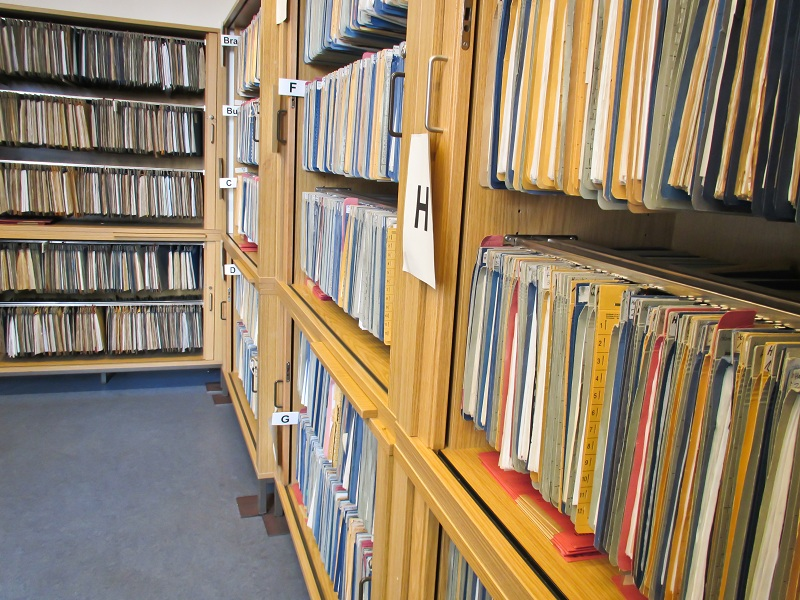
\includegraphics[scale=1.5]{resourse/folders-archivos.jpg}
    \caption{Almacenamiento Fisico de Archivos}
    \label{fig:05}
\end{figure}  


\begin{figure}[H]
    \centering
    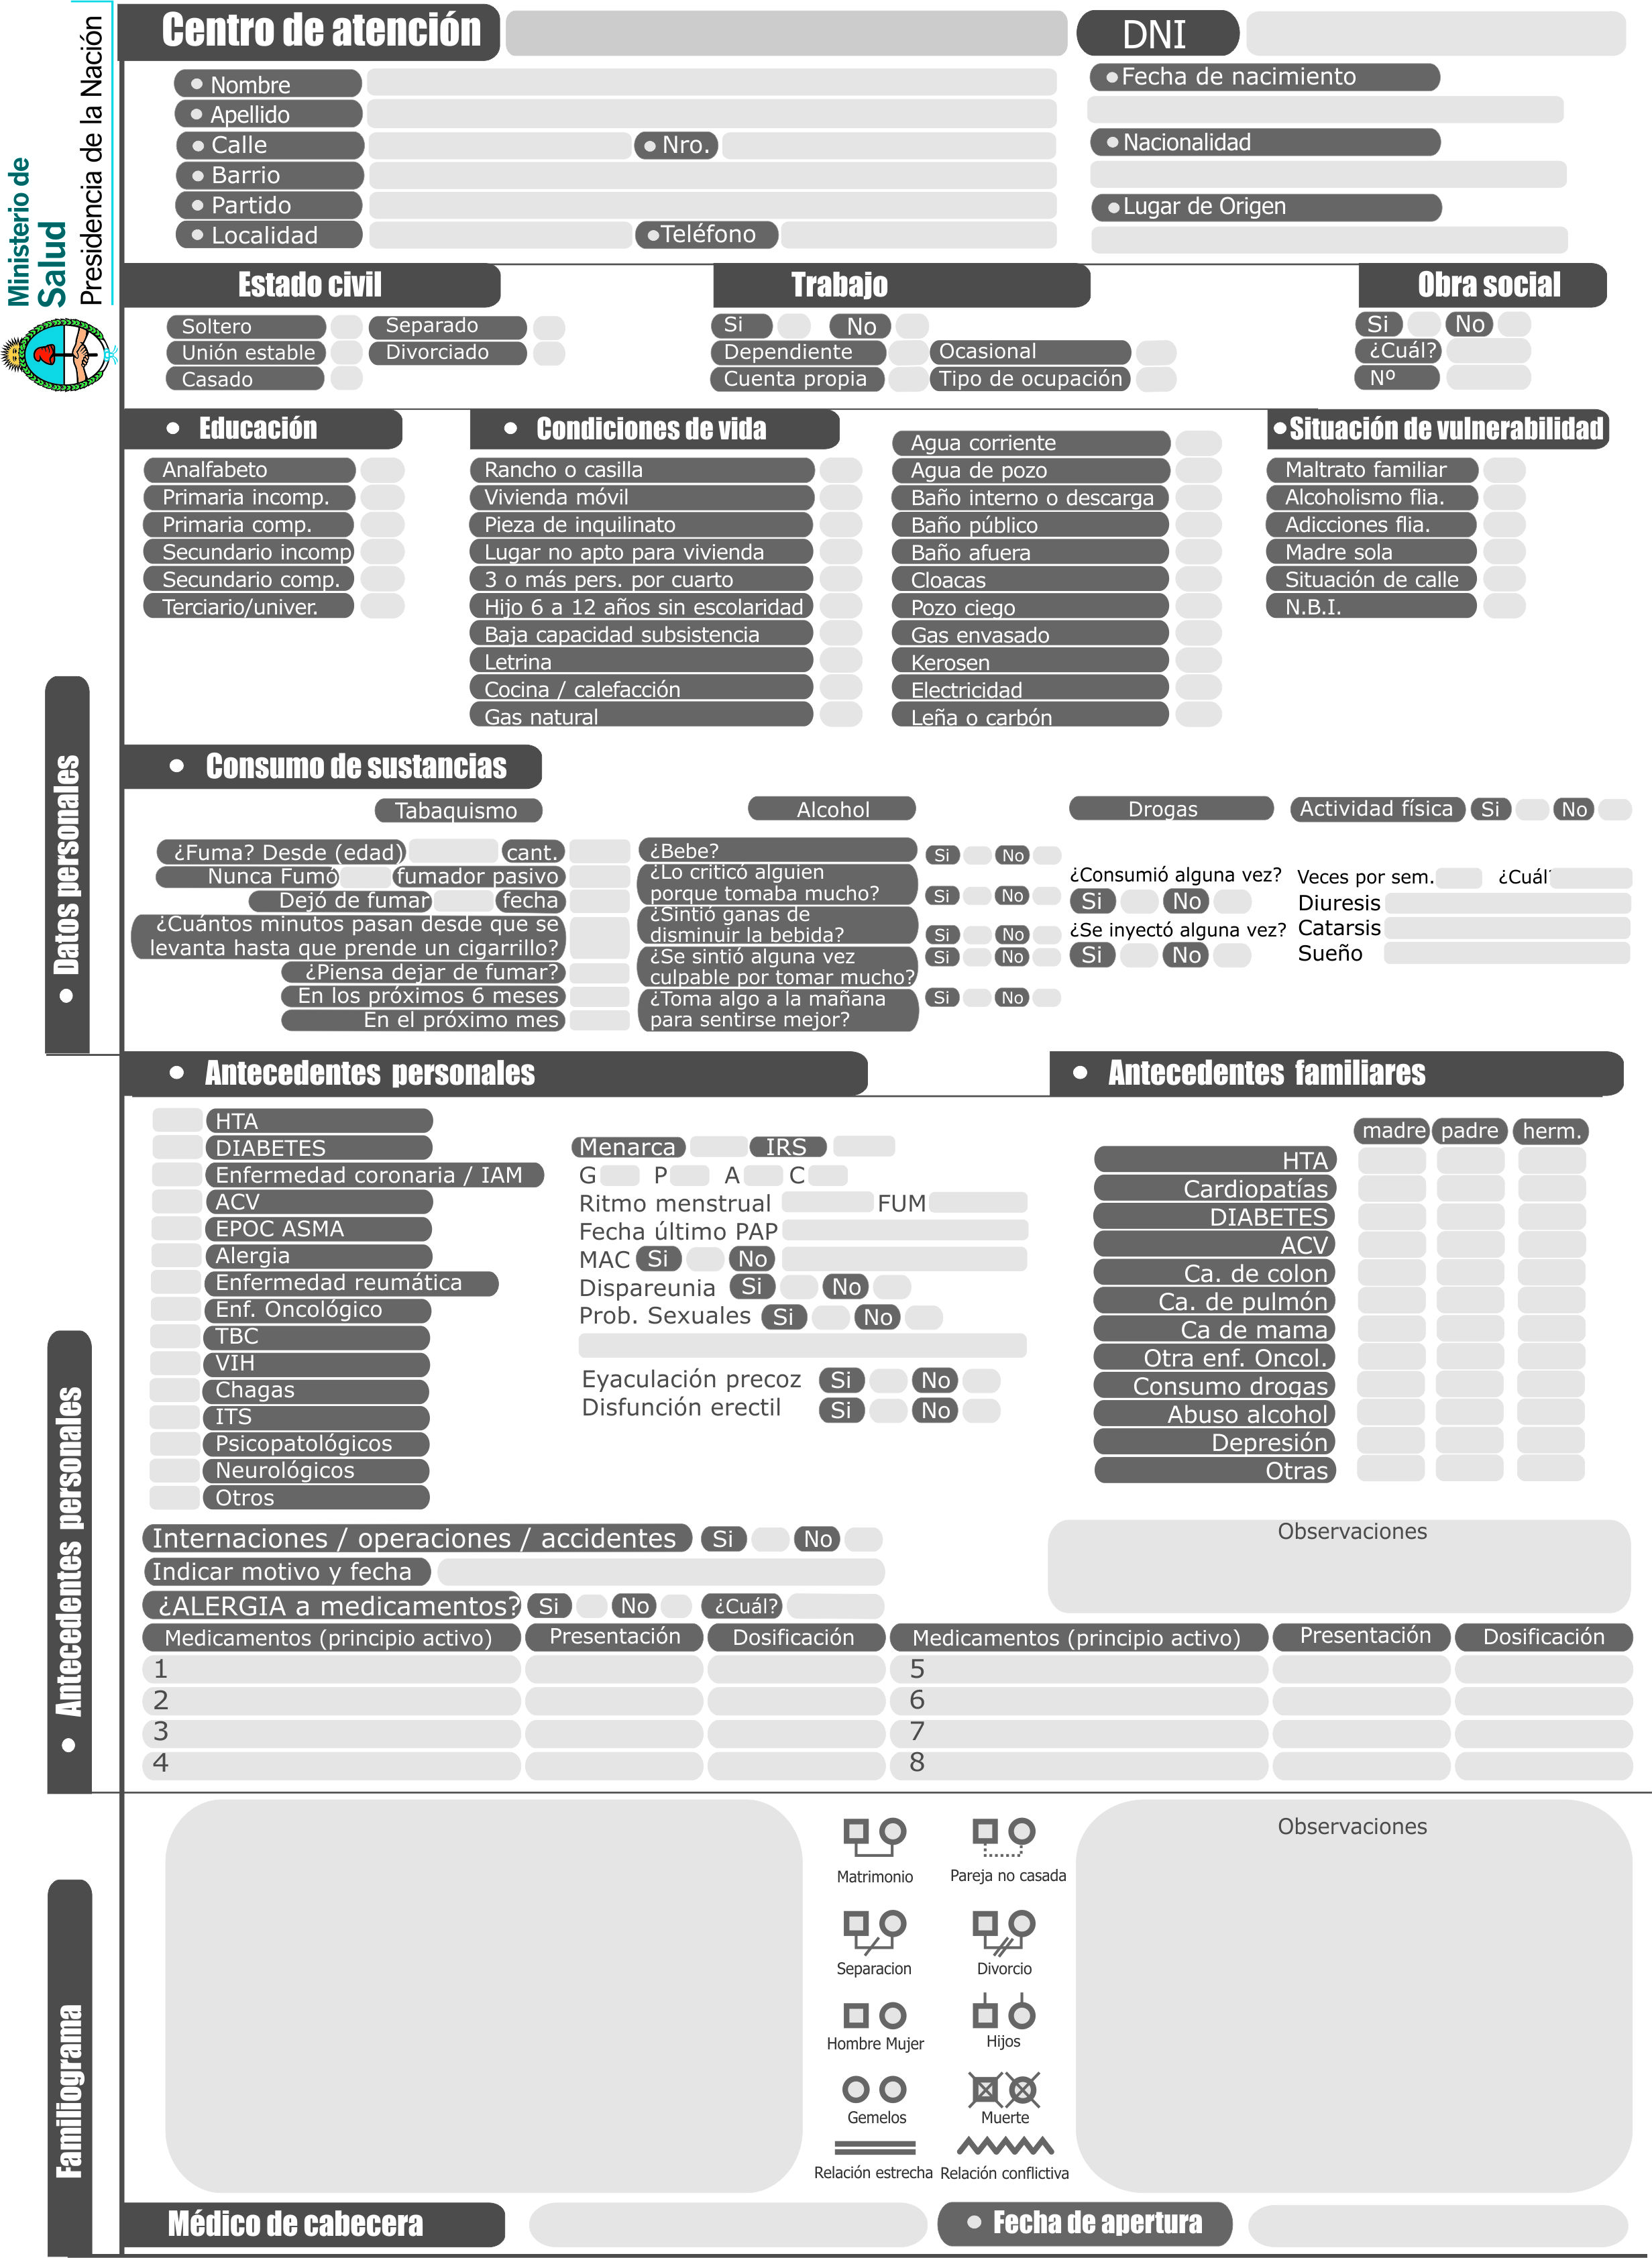
\includegraphics[scale=0.7]{resourse/historia-clinica-f.jpg}
    \caption{Modelo Historia Clinica Ministerio de Salud de La Nacion Pag 1}
    \label{fig:06}
\end{figure}  

\begin{figure}[H]
    \centering
    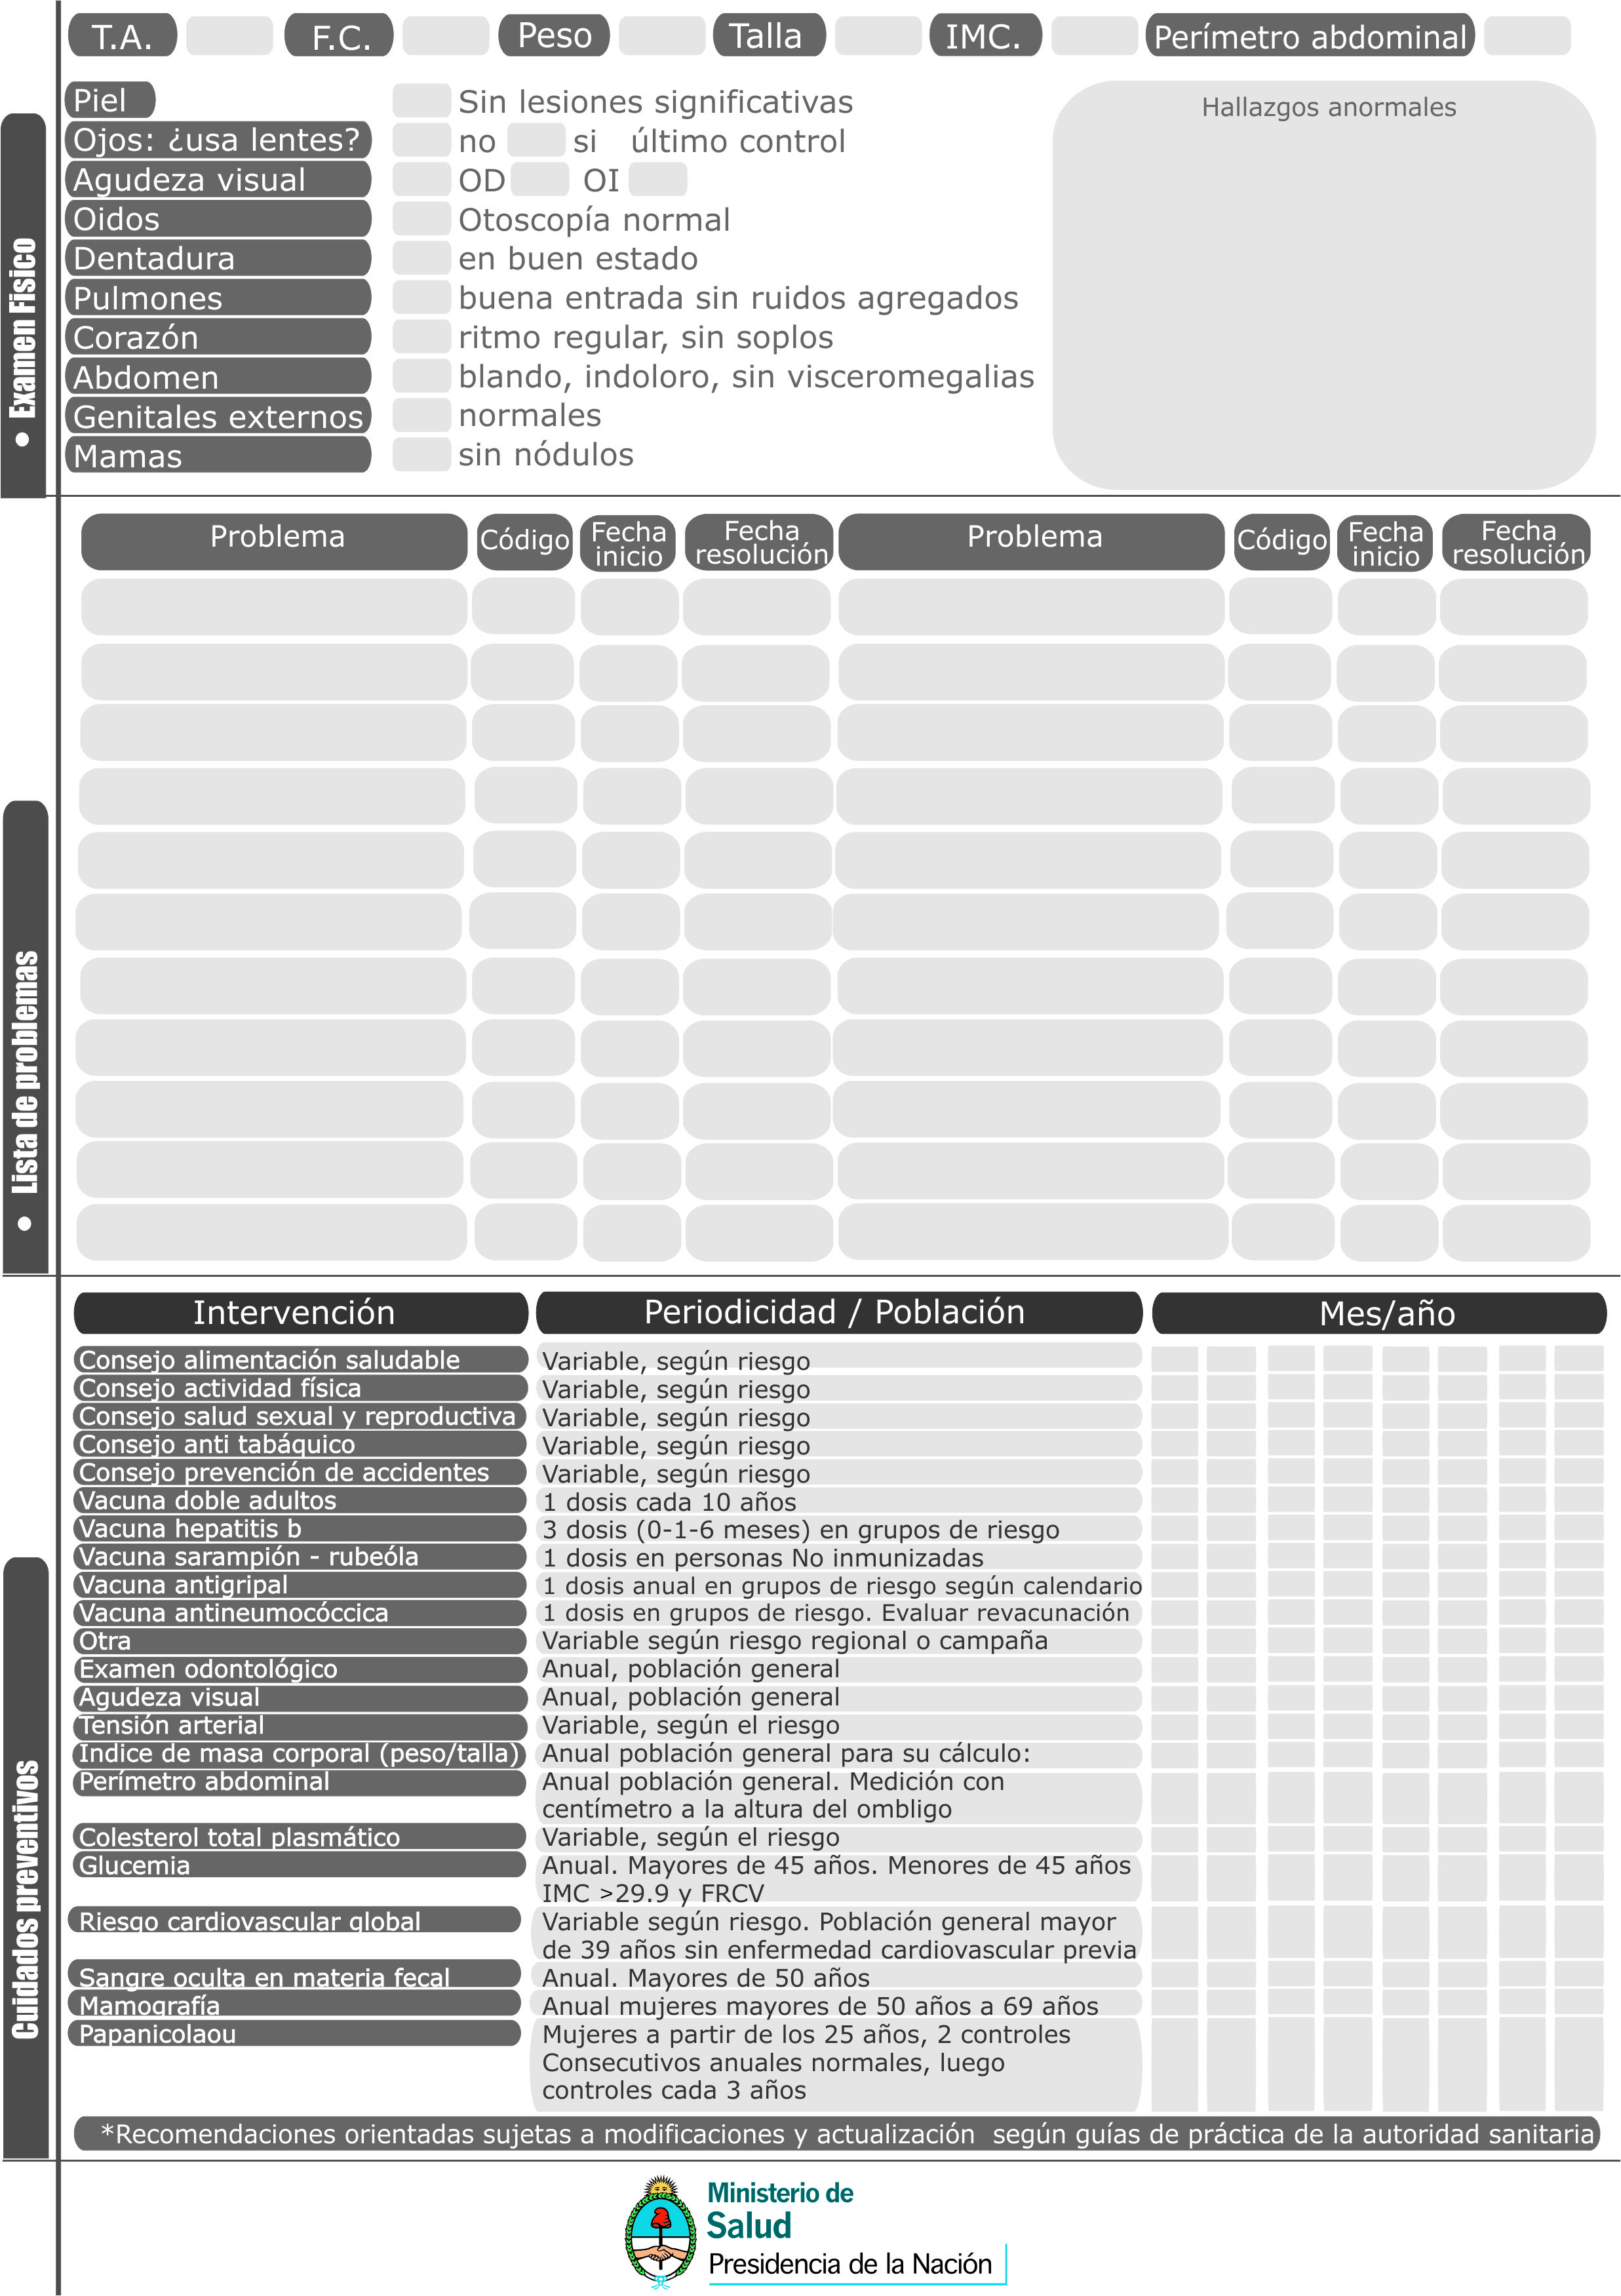
\includegraphics[scale=0.7]{resourse/historia-clinica-d.jpg}
    \caption{Modelo Historia Clinica Ministerio de Salud de La Nacion Pag 2}
    \label{fig:07}
\end{figure}

\section{Problemas del Sistema Actual}


\subsection{Almacenamiento}
 A medida que crece el numero pacientes y la informacion que va
anexando a cada Archivo se va necesitando mas espacio fisico para almancenar
dicha informacion. Por ello con el paso del tiempo las instalaciones dedicadas
a tal fin suelen verse colapsadas por los grandes volumenes de informacion que
deben manejar.\\[0.1cm]

\subsection{Busqueda y Localizacion}
La Busqueda de expedientes se puede agilizar un poco utilizando una buena organizacion,
el problema es que la mayoria de los edificios para tal fin, suelen estar saturados
por grandes volumenes de archivos fisicos, Por lo que encontrar un archivo requerido
suele ser una tarea costosa y lenta.\\[0.1cm]

\subsection{Deterioro}
En lo que hace a la conservación propiamente dicha, el combate de los
problemas habituales que se derivan de las condiciones climáticas, de la humedad,
de las plagas, del deterioro natural del papel, especialmente por su fabricación
con celulosa desde hace dos siglos, es una constante que, pese a sus avances,
no ha encontrado soluciones definitivas. Por ende, una preocupación común a los
archivos y bibliotecas, es encontrar remedios prácticos y asequibles para
asegurar la preservación de sus acervos. De lo anterior se desprende la
necesidad, en el nivel nacional, de procurar el establecimiento de políticas y
normas sobre conservación en las instituciones públicas y privadas dedicadas
a la protección del patrimonio.\\[0.1cm]

\subsection{Otros Poblemas}
Otros problemas que acarrean el uso de archivos fisicos son:

\begin{itemize}
    \item Pérdida, alteración o daño de documentos importantes
    \item Gasto excesivo en fotocopias
    \item Altos costos de personal para administrar, suplir, mantener y recuperar el archivo físico
    \item Costos asociados al transporte de documentos ya sea interna o externamente
    \item Costos asosiados al espacio físico requerido para su almacenamiento
    \item Falta de condiciones adecuadas para el almacenamiento de documentos como: ventilación, humedad, temperatura
    \item Falta de respaldo adecuado en caso de catastrofe como incendio, inundación o terremoto
\end{itemize}


\subsection{La Solucion Planteada}

Por ello este era un ecenario perfecto donde Es Necesario informatizar el
Actual Sistema, lo cual solucionaria los 2 principales problemas del mismo
que son el Excesivo espacio de almacenamiento y el lento trabajo de busqueda
ademas de:

\begin{itemize}
    \item Reducir costos de Personal Administrativo, ya que las busquedas y
    registro las hara el Sistema.
    \item Brindar la informacion de manera rapida en situaciones criticas que
    requieren un rapido accionar por parte del Medico.
   \item Disponibilidad En todo momento y cualquier lugar para consulta por
    parte de los Medicos ya que solo requerira disponer de un usuario y un
    ordenador con coneccion a Internet para poder consultar.
\end{itemize}

Es cierto que los sistemas informaticos sufren problemas de Almacenamiento, Busqueda
(en el caso de grandes volumenes de informacion) y deterioro por el paso del tiempo
Pero en este caso el primero se soluciona Agregando mas espacio de disco, cosa que
hoy en dia es algo relativamente barato a razon de 1 peso = 1 Gb. \footnote {Gb hace referencia a
Gigabyte que es una medida utilizada en informatica la cual normalmente hace referencia
a tama\~nos de almacenamiento.}  \\[0.1cm]

El problema de las busqueda no afecta mucho con la velocidad de los equipos
actuales se puede consultar bases de datos con millones de registro en unas
pocas milesimas de segundos dicho tiempo resulta impersectible para la persona
en la mayoria de las veses, en todo caso dependera de la implementacion y el
motor de bases de datos mas que de las prestaciones del hardware.\\[0.1cm]

En cuanto al deterioro, puede que con el tiempo los equipos de hardware
tales como discos duros fallen en algun momento, pero esto es salvable siempre y
cuando se realizen buenas practicas tales como implementar un sistemas de backup,
tambien replicacion de datos en caso de que se necesite alta disponibilidad de
la informacion que se almacena.\\[0.1cm]


\section{Gestion de Turnos}   

En lo que respecta a asignacion de turnos, el sistema actual en la mayoria de
los casos no ha tenido un mejor panorama en cuanto a implatancion de un software,
aunque ya en esta area existen algunas aplicaciones que intentan solucionar el
problema de manera mas o menos eficientes.\\[0.1cm]
























\chapter{El Proyecto}


\section{Motivaci\'on}

En la actualidad existen pocos sistemas Aplicados en el \'ambito de la gesti\'on en
el area de Medicina y los existentes suelen ser solo para areas especificas


\section{Descripci\'on del Proyecto}

Lo que se pretendi\'o con este proyecto era poder desarrollar un sistema que unifique
la areas de gesti\'on y asignaci\'on de turnos y el manejo de historia cl\'{\i}nica en 
un \'unico sistema.

Cabe aclarar que el mismo se desarrollo con el prop\'osito de poder ser utilizado 
principalmente en policonsultorios m\'edicos ya que no plantea cuestiones tales como
internaciones, traslado de pacientes, etc. como para poder ser de correcta utilidad
en cl\'{\i}nicas y hospitales. 


\section{Arquitectura de la Aplicaci\'on}

Implementado en Python utilizando en Framework Django, utilizando el motor de bases
de datos PosgreSQL, funciona con una interfaz web por lo que se se accede al
mismo mediante un Navegador Web, Internamente maneja 2 Modulos principales
que son el  ``Modulo de Gesti\'on de Turnos" y el ``Modulo de manejo de
Historia Cl\'{\i}nica" , al ser un sistema web implementa un tercer modulo de manera
impl\'{\i}cita que control de acceso mediante la definici\'on de Grupos Usuarios y
sus correspondientes permisos.


\section{Modulo Usuarios}

La gesti\'on de usuarios es un proceso bastante com\'un en casi todos los sistemas,
muchos desarrolladores terminan programando funcionalidades de autenticaci\'on 
una y otra ves a lo largo de los a\'nos y casi siempre funcionando de la misma 
manera. Django se pens\'o para simplificar la vida no para complicarla, por eso
al ser una tarea bastante com\'un en casi todas las aplicaciones, viene incluido
un completo sistema de autenticaci\'on que gestiona:

\begin{itemize}
    \item Usuarios
    \item Grupos
    \item Permisos
    \item Sessiones de Usuarios y Cookies
\end{itemize}

Aunque en cuanto a lo que se refiere manejo de sesiones es un completo sistema
solo maneja un peque\~no conjunto de datos por lo que hubo que extender mediante 
la adici\'on de un Modelo adicional para complementar la informaci\'on de los 
usuarios.


\subsection{Modelos}

Aqui un diagrama con todos los modelos que componen el modulo Usuarios.

\begin{figure}[H]
    \centering
    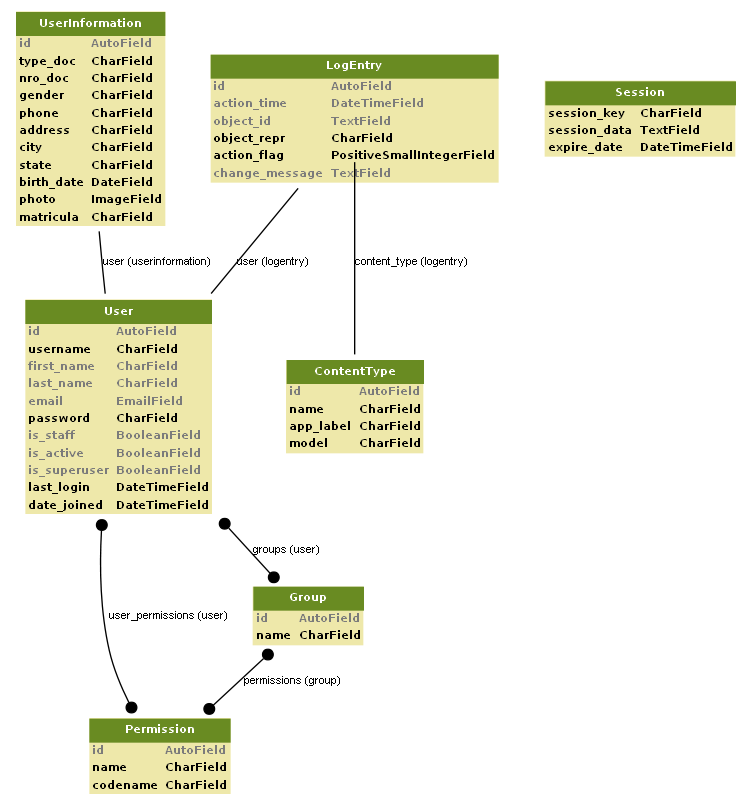
\includegraphics[scale=0.6]{resourse/auth.png}
    \caption{Diagrama con modelos que componen el modulo Usuarios}
    \label{fig:07}
\end{figure}

%Si lo expres\'aramos mediante la notaci\'on UML para Diagramas de Clases 
%tendr\'{\i}amos lo siguiente.
%
%\begin{figure}[H]
%    \centering
%    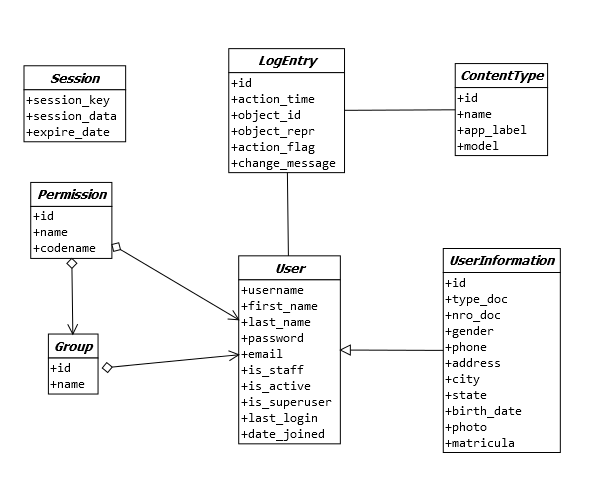
\includegraphics[scale=0.7]{resourse/uml-users.png}
%    \caption{Diagrama con modelos que componen el modulo Usuarios}
%    \label{fig:07}
%\end{figure}

El \'unico modelo que fue necesario agregar es UserInformation que es para 
extender la informacion que se registra en el Modelo User el resto vienen
con Django. En Resumen aunque se podr\'{\i}a haber desarrollado Un Modulo desde
cero que gestione las sesiones de usuarios hubiese generado trabajo extra sin
sentido.

\subsection{Usuarios y Permisos}

El sistema contempla 4 tipos de usuarios los cuales son: 

\begin{itemize}
    \item Usuarios no registrados 
    \item Pacientes
    \item M\'edicos
    \item Administrativos
\end{itemize}

\subsubsection{Usuarios no Registrados}

Los \textbf{Usuarios no registrados} que vendr\'{\i}a a ser cuando el usuario ingresa
a la aplicaci\'on y no hay ninguna sesi\'on iniciada, pueden acceder al sistema para 
consultar informaci\'on b\'asica y horarios de atenci\'on de los especialistas que 
forman parte de la instituci\'on, adem\'as de tener la opci\'on de registrarse 
como paciente.\\[0.1cm]    

\subsubsection{Paciente}

El rol \textbf{Paciente} corresponde a los usuarios comunes, un usuario paciente puede 
ser creado por cualquiera de los otros roles, en caso que sea un usuario no registrado
quien da el alta como paciente, el mismo deber\'a confirmar el registro mediante un
codigo de verificaci\'on que el sistema le enviara al correo antes de poder comenzar
a usar su cuenta, en los otros casos (el usuario Paciente es registrado por un 
medico o un Administrativo) no se requerida dicha confirmaci\'on.\\[0.1cm]

En cuanto a los privilegios del usuario Paciente, este adem\'as de poder consultar la 
la informaci\'on de los especialistas puede solicitar un turno para ser atendido 
a un especialista en particular, tambi\'en realizarle una interconsulta (mediante
el sistema interno de mensajer\'{\i}a) y modificar sus datos b\'asicos, en resumen sus 
posibles funciones son:


\subsubsection{Medico}

Los Usuarios \textbf{M\'edicos} los cuales son asignados por los Administrativos a 
los Especialistas, en cuanto a privilegios y funcionalidades dentro del sistema, 
los mismos pueden:

\begin{itemize}
    \item Registrar Pacientes
    \item Modificar datos de Pacientes
    \item Enviar Mensajes a cualquier Usuario
    \item Registrar Turnos 
    \item Cancelar Turnos
    \item Administrar sus Horario de Atenci\'on
    \item Cancelar d\'{\i}as de atenci\'on
\end{itemize}

Son los \'unicos usuarios que tienen acceso al Modulo \textit{Historia Clinina}, en cuanto
a privilegio sobre este modulo diremos que tiene la posibilidad de Crear,Modificar,
Borrar (salvo casos espec\'{\i}ficos, que por su naturaleza no se permite dicha 
modificaci\'on.) un conjunto de Estudios, para mas detalle se recomienda consultar
el apartado sobre tal modulo.


\subsubsection{Administrativo}

En cuanto a los usuarios \textbf{Administrativo} poseen los mismos permisos que 
un usuario \textbf{Medico} exceptuando que no poseen acceso a las funcionalidades 
del Modulo Historia Cl\'{\i}nica, como privilegio especial pueden administrar las 
cuentas de usuario de todos los roles incluidos en el sistema, incluido los 
Medico y otros Administrativos.

\subsubsection{Admin}

Existe un rol adicional que Django crea y gestiona por aparte, el mismo queda 
delegado para los administradores del sistemas ya que mediante el se puede acceder
y modificar cualquier parte de la base de datos, por lo que podr\'{\i}amos decir que 
es un \textbf{Super Usuario}, o usuario \textbf{Root} como para hacer analog\'{\i}a
con los usuarios en entornos Unix, el mismo no forma parte del sistema desarrollado
sino como funcionalidad adicional Django provee un panel de administraci\'on, 
para dicho tipo de usuario, al cual se puede acceder desde \url{/admin/} por ejemplo
si estuvi\'esemos ejecutando en un servidor local la ruta completa seria 
\url{http://127.0.0.1/admin/}\footnote{Se puede consultar mas acerca de Django
Admin en \url{https://docs.djangoproject.com/en/dev/ref/contrib/admin/}}.\\[0.1cm]


\begin{figure}[h]
    \centering
    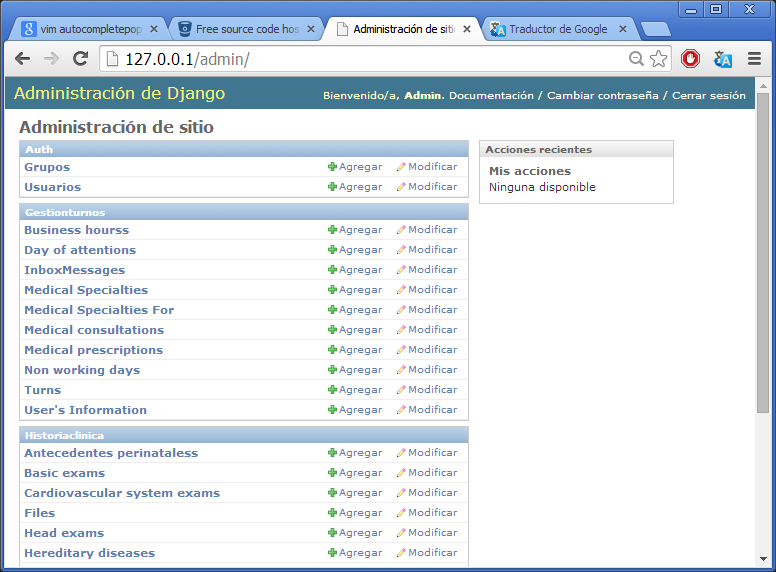
\includegraphics[scale=0.5]{resourse/django-admin.png}
    \caption{Vista del Panel Administracion provisto por Django}
    \label{fig:123}
\end{figure}  


Cabe aclarar que el Super Usuario del sistema de Autenticaci\'on de Django dentro 
del sistema en si mismo no posee ning\'un privilegio adicional, es mas para 
compatibilizar el usuario con la funcionalidad del sistema, cuando se inicializan
por primera ves, se crea un usuario de este tipo llamado \textbf{admin} al cual
se le asignan privilegio de \textit{Administrativo}.


%%%%%%%%%%%%%%%%%%%%%%%%%%%%%%%%%%%%%%%%%%%%%%%%%%%%%%%%%%%%%%%%%%%%%%%%%%%%%%%

\section{Modulo Gesti\'on de Turnos}

Dejando de lado el modulo Usuarios que nos provee Django el sistema desarrollado 
se divide esencialmente en 2 partes o m\'odulos, aqu\'{\i} explicare como se dise\~no e
implemento el Modulo Gesti\'on de Turnos, que a mi consideraci\'on fue el que mayor
reto aporto a la hora de pensar un soluci\'on para poder implementarlo.

El modulo se encarga de implementar las siguientes funciones

\begin{itemize}
    \item Gestionar Datos de Usuarios
    \item Mensajer\'{\i}a Interna
    \item Asignacion de Especialidades Medicas
    \item Asignaci\'on de Turnos
\end{itemize}


\subsection{Definicion del Modelo}

Aqui se muestra el diagrama de modelos que componen el modulo \textbf{Gestion 
de Turnos} \footnote{Vuelven a aparecen los modelos User y UserInformation por 
que casi todos los otros modelos dependen de alguna forma de ellos}, por la 
cantidad de modelos se mostrara en 2 diagramas, igualmente tengase en cuenta
que corresponden a un unico modelo, lo que haremos sera separar en los modelos
especificos utilizados para gestion de turnos y el resto de los modelos 
definidos que complementan la funcionalidad del modulo.

Por Cuestiones de tamaño del diagrama y por la cantidad modelos utilizados en 
el modulo se complicaba poder mostrarlos todo en una misma pagina por lo que 
para mejor visualizacion e interpretacion separe el mismo en 2 partes:

El primer diagrama unifica todo lo referente a la asignacion de turnos, que es lo 
principal del modulo:

\begin{figure}[H]
    \centering
    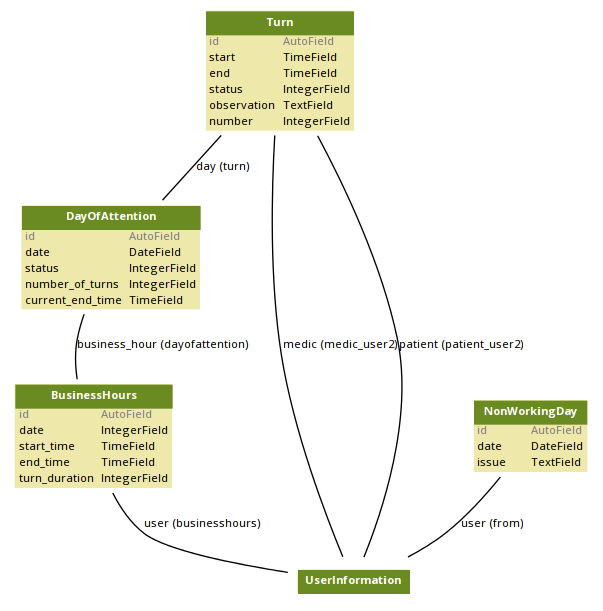
\includegraphics[scale=0.6]{resourse/gt-gt.png}
    \caption{Modulo Gestion Turnos - Diagrama Modelos correspondiente a la Gestion de Turnos}
    \label{fig:124}
\end{figure}  

En el segundo diagrama se muestra los modelos necesarios para las funcionalidades 
adicionales.

\begin{figure}[H]
    \centering
    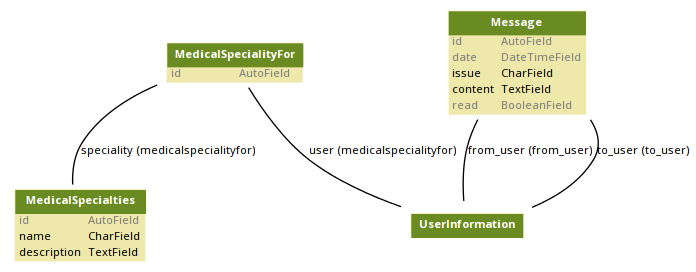
\includegraphics[scale=0.6]{resourse/gt-ot.png}
    \caption{Modulo Gestion Turnos - Modelos Adicionales}
    \label{fig:125}
\end{figure}  


\subsection{Gestionar Datos de Usuarios}

Esta funcionalidad describe, todo lo referido a la alta, baja y modificaci\'on de 
los datos de todos los usuarios. Implementa las vista tanto para modificacion de 
datos personales, vistas de administrador para gestionar datos de otros usuarios. 


\subsection{Mensajer\'{\i}a Interna}

Permite la comunicacion interna entre los usuarios, su principal utilidad es 
permitir que los Pacientes puedan realizar peque\~nas interconsultas a los 
medicos atraves de la plataforma, sin requerir una consulta medica.

\subsection{Asignacion Expecialidades Medicas}

Dentro el modulo permite asignarles especialiades medicas correspondientes a 
a los profesionales, aunque no realiza una distincion especifica a la hora de 
asignar turnos, simplemente considera que el medico en dicho horario puede 
atender cualquier consulta relacionada a sus especializaciones. \footnote{
Tengase en cuenta que es raro ver un medico con varias especializaciones Medicas
y que el sistema fue pensado para ser utilizado en un consultorio medico, donde
no se suele contar con equipamiento de alta complejidad.}


\subsection{Asignaci\'on de Turnos}  

La \textit{Asignacion de Turnos} al los pacientes es la principal funcionalidad 
del modulo, que entre otras funcionalidades permite:

\begin{itemize}
    \item Definir dias de atencion
    \item Definir dias feriados o de Vacaciones     
    \item Asignar turnos
    \item Controlar la asistencia de los pacientes.    
\end{itemize}

%\\[0.5cm]

\subsection{Dise\~no de Modelos Para la Gestion de Turnos}

Aqui se muestran los algunas consideraciones que se tubieron en cuenta a la hora de 
dise\~nar los modelos para implementar la funcionalidad de asignacion de turnos
propiamente dicha la cual define el nombre del modulo. 


\subsubsection{BussinesHour(Horario De Atencion)}

Este modelo se utiliza para definir el horario de atencion de cada medico, en 
el se especifican parametros como:

\begin{itemize}
    \item \textbf{user}: referencia al medico al cual pertence 
    \item \textbf{date}: define el dia de atencion \footnote{Esto hace 
        referencia a los dias de la semana osea Lunes, Martes,..., etc. por el 
        momento solo se puede definir un unico dia de atencion por dia por 
    medico.}
    \item \textbf{start\_time, end\_time}: marca el horario de inicio y fin del 
        dia de atencion del medico.
    \item \textbf{turn\_duration} duracion estimada del turno
\end{itemize}

En base a esto se puede calcular un dato adicional que es la cantidad de turnos
que se pueden asignar en tal dia, y se hace de la siguiente manera:

\begin{lstlisting}
numero\_turnos = (hora\_fin - hora\_inicio) // turn\_duration
\end{lstlisting}

Esto devolvera un valor entero, que sera el numero maximo de turnos que se 
puedan asignar.


\subsubsection{DayOffAttention (Dias de Atencion)}

Este modelo maneja la disposicion horaria de una fecha en particular, se basa 
en los datos que se definieron en el modelo anterior BussinesHour, por lo que 
solo se pueden generar en las fechas que correspondan con los dias de la semana
asignados, cuenta con los siguientes parametros:

\begin{itemize}
    \item \textbf{bussines\_hour}: referencia al horario de atencion definido 
        por el medico.
    \item \textbf{date}: que fecha cae ese dia, esto se refiere al dia del a\~no 
        especifico.
    \item \textbf{status}: informacion del estado del dia, es de tipo booleano
        y especifica el estado del dia de atencion siendo el valor true 
        para explicar que se pueden asignar mas turnos y FALSE que no se 
        pueden asignar mas. \footnote{ Que un dia de atencion este marcado como 
        no disponible (status=FALSE) puede significar que el cupo este lleno o 
        que ese dia el medico no pueda asistir o sea feriado por ejemplo, para 
        determinar de que se trata si dice no disponible y no hay ningun turno 
        asignado (number\_of\_turns=0) significara que ese dia el medico no 
        atiende }
     \item \textbf{number\_of\_turns}: numero de turnos que van siendo asignados
     \item \textbf{current\_end\_time}: horario actual de finalizacion 
\end{itemize}


\subsubsection{Turn (Turno)}

Este modelo se define para registrar la informacion correspondiente a los 
turnos asignados es dependiente del modelo anterior (DayOffAttention) donde se 
especifican el resto de los datos como la fecha.

En cuanto a sus atributos, mucho no hay que explicar y son:

\begin{itemize}
    \item \textbf{day}: hace referencia a un dia de atencion (DayOffAttention)
    \item \textbf{medic}: referencia a los datos del medicos
    \item \textbf{patient}: referencia al paciente. 
    \item \textbf{start, end}: hacen referencia a las horas de inicio y fin 
        correspondientemente.
    \item \textbf{status}: estado del turno es de tipo enumerado define varios 
        posibles estados entre los que estan (pendiente, concretado, cancelado 
        medico, cancelado paciente).
    \item \textbf{observation}: campo de texto, para registrar cualquier 
        observacion pertinente.
    \item \textbf{number}: se refiere al numero de orden para atencion.
\end{itemize}


\subsubsection{Consideraciones}

En cuanto a funcionamiento de la asignacion de turnos se tienen en cuenta las
siguientes consideraciones: \\[0.1cm]

Un turno no puede ser cancelado despues de su hora de inicio por el paciente, 
siendo asi posible de ser cancelado por el medico. \\[0.1cm]

Al ser cancelado por un paciente se debe cambiar correspondiente estado dentro 
de dia de atencion. \\[0.1cm]

 Si un medico cancela un turno el mismo no se modificara el estado en la tabla 
 dia de atencion, como el caso de los paciente que cancelen un turno, 
 para el sistema hara de cuenta que los mismo ocurrieron, aunque si un turno es 
 cancelado por el medico el mismo no sera reprogramado.

 En todos los casos los usuarios deverian poder recivir el correspondiente 
 notificacion de que se cancelo dicho turno invitandolos a reprogramar el mismo.

Los pacientes no pueden solicitar turnos durante el horario de atenci\'on del 
mismo, si el servidor comprueba que existen turnos sin actualizar estado como 
pendientes, si el medico o administrador no actualizo los msmos y ya paso la 
hora del mismo tiene que enviar notificaciones correspondientes. 


%%%%%%%%%%%%%%%%%%%%%%%%%%%%%%%%%%%%%%%%%%%%%%%%%%%%%%%%%%%%%%%%%%%%%%%%%%%%%%

\section{Modulo Historia Cl\'{\i}nica}

Este modulo del sistema tiene como tarea manejar y recolectar toda informaci\'on 
referente a las historia cl\'{\i}nica de los pacientes.


\subsection{?`Que es una Historia Cl\'{\i}nica?}

Antes de entrar en todo lo referente sobre el desarrollo del correspondiente modulo
tomo un momento para explicar concretamente a que no referimos cuando hablamos de 
la misma por lo que aqu\'{\i} tenemos la siguiente definici\'on:

La historia cl\'{\i}nica es un documento m\'edico-legal que surge del contacto entre el 
profesional de la salud (m\'edico, pod\'ologo, psic\'ologo, asistente social, enfermero, 
kinesi\'ologo, odont\'ologo, etc.) y el paciente donde se recoge la informaci\'on necesaria 
para la correcta atenci\'on de los pacientes. La historia cl\'{\i}nica es un documento 
v\'alido desde el punto de vista cl\'{\i}nico y legal, que recoge informaci\'on de tipo 
asistencial, preventivo y social.

La Historia Cl\'{\i}nica se origina con el primer episodio de enfermedad o control de salud en 
el que se atiende al paciente, ya sea en el hospital o en el centro de atenci\'on primaria, 
o en un consultorio m\'edico. La historia cl\'{\i}nica est\'a incluida dentro del campo de la 
semiolog\'{\i}a cl\'{\i}nica \footnote{La Semiolog\'{\i}a Cl\'{\i}nica es el cuerpo del conocimiento
que se ocupa de la identificaci\'on de las diversas manifestaciones patol\'ogicas 
\cite{SemiClin}}.

\subsection{La Historia Cl\'{\i}nica en la Ley Argentina}

La documentaci\'on m\'edica comprendida en lo que com\'unmente se denomina ``historia 
cl\'{\i}nica" la cual no se encontraba regida por leyes especificas en la Argentina hasta
el 19 de noviembre del 2009 donde se promulga la Ley 26.529 \cite{LeyHC}.\\[0.1cm]

En el cap\'{\i}tulo primero de la ley sen enumeran los derechos de los pacientes, 
en el art\'{\i}culo 2, inciso ``a". Renueva el derecho a la intimidad y la confidencialidad, 
donde se hace hincapi\'e sobre la responsabilidad de preservar la intimidad y 
confidencialidad de toda la documentaci\'on m\'edica concerniente a los pacientes, 
particularmente el inciso ``d" del mismo art\'{\i}culo:\\[0.1cm]

``El paciente tiene derecho a que toda persona que participe en la elaboraci\'on 
o manipulaci\'on de la documentaci\'on cl\'{\i}nica, o bien tenga acceso al contenido de 
la misma, guarde la debida reserva, salvo expresa disposici\'on en contrario 
emanada de autoridad judicial competente o autorizaci\'on del propio paciente".\\[0.1cm]

Garantiza adem\'as el respeto por la autonom\'{\i}a del paciente y el derecho a recibir 
la informaci\'on necesaria para su salud, incluyendo el derecho a negarse a ser 
informado.\\[0.1cm]

El cap\'{\i}tulo III reza sobre el Consentimiento Informado, el cual est\'a basado en 
el principio de autonom\'{\i}a, es decir, el derecho del paciente a ser reconocido 
como persona libre y due\~na de tomar sus decisiones. Para ello el paciente debe estar en 
condiciones de comunicar su decisi\'on y  \'este ha sido informado adecuadamente de 
sus opciones, es decir, no pueden ser decisiones hechas como resultado de delirio 
o alucinaciones. La decisi\'on del paciente es consistente con sus valores y metas 
y se mantiene estable en el tiempo si no han habido modificaciones hechas por
el mismo sujeto. Los familiares de un paciente no est\'an en el derecho de 
requerir al m\'edico del paciente que no se le comunique ciertos detalles o
informaci\'on al mismo. \\[0.1cm]

Ahora bien vallamos a lo que nos interesa:\\[0.1cm]

La ley define a la Historia Cl\'{\i}nica como el documento ``obligatorio, cronol\'ogico,
foliado y completo en el que consta toda actuaci\'on realizada al paciente por
profesionales y auxiliares de la salud." Define que la historia cl\'{\i}nica es 
propiedad del paciente, siendo este el titular de la misma. Siempre que un paciente 
solicite la historia cl\'{\i}nica, la instituci\'on competente debe entregarle una copia
autenticada en 48 horas. Si no es entregada en ese plazo, el
paciente est\'a autorizado a interponer un recurso de Habeas Data, juzgado de por 
medio. \\[0.1cm]

Entre los datos que han de consignarse en forma obligatoria esta la fecha de 
inicio y confecci\'on de la historia cl\'{\i}nica, datos identificatorios del paciente
y su n\'ucleo familiar, datos del profesional interviniente y su especialidad, 
registros claros y precisos de los actos realizados por profesionales y auxiliares
intervinientes, antecedentes gen\'eticos, fisiol\'ogicos y patol\'ogicos si los hubiere,
y todo acto m\'edico realizado o indicado.\\[0.1cm]

Incluye en la historia cl\'{\i}nica a todos los documentos que hagan referencia a 
informaci\'on de salud del paciente, a\~nadiendo los consentimientos informados, 
hojas de indicaciones, hojas de enfermer\'{\i}a, estudios complementarios, 
incluyendo las``pr\'acticas realizadas, rechazadas o abandonadas." 
Esto  \'ultimo es interesante: si el paciente abandona o rechaza un tratamiento 
propuesto, es responsabilidad del m\'edico consignarlo, que a fin de cuentas es el
beneficiario de que aquello quede asentado desde el punto de vista m\'edico-legal.\\[0.1cm]

Autoriza a reclamar una copia de la historia cl\'{\i}nica al paciente y su representante 
legal, al c\'onyuge o conviviente de hecho (sin importar el sexo), y a los herederos 
forzosos. Lo que no queda claro del art. 19 inciso b es si los c\'onyuges y 
convivientes requieren o no la autorizaci\'on del paciente.\\[0.1cm]

Se a\~nade esta ley al cap\'{\i}tulo 11 del C\'odigo de \'etica de la Asociaci\'on M\'edica 
Argentina, del a\~no 2001. En ella se explaya en forma m\'as extensa y detallada sobre
la confecci\'on. Particular inter\'es debi\'eramos prestarle al art. 168:\\[0.1cm]

``La historia cl\'{\i}nica ha de ser un instrumento objetivo y comprensible por terceros,
y no solo por quienes escriben en ella." A su vez, el art. 171 especifica que 
"debe ser legible, no debe tener tachaduras, no se debe escribir sobre lo ya 
escrito, no debe ser borrada, no se debe dejar espacios en blanco y ante una
equivocaci\'on debe escribirse ERROR y aclarar lo que sea necesario. No se debe a\~nadir
nada entre renglones."


\subsection{Funcionalidades}

Las funcionalidades que se implementan en correspondiente m\'odulos son solo
b\'asicas y comprenden la documentaci\'on practicas mas comunes dentro del area de la 
medicina, esto no implica que solo valla a servir para eso \'unicamente, por su 
extructura el modulo contempla la posibilidad de agregar nuevos componentes para 
estudios especificos que sean requeridos y que no hayan sido contemplados en el 
actual sistema.\\[0.1cm]


El modulo se encarga basicamente de registrar los diferentes estudios que se le 
practican a un paciente, adicionalmente registra informacion correspondiente a 
las interconsultas \footnote{Consultas medicas realizadas por el paciente} y las
observaciones del medico, asi como los medicamentos que fueron recetados por el 
especialista.


\subsection{Definicion de Modelos}

Los modelos que componen el Modulo corresponden a los diferentes tipos de 
Examenes de practica mas comun\footnote{Esto no es que este definido en algun 
lado que sean solo estos, sino que mas bien son los examenes que durante el 
analisis de diferentes modelos se presentaban mas comunmente.} en lo que 
corresponden a Historia Clinica.\\[0.1cm]

Aqui tambien por la cantidad de modelos se hace dificil poder colocarlos todos 
en un unico diagrama dentro de la pagina por lo que tambien se separara en 
varias partes sin romper las relaciones de los mismo, osea aunque se realize 
una separacion de los mismos corresponden a un unico modulo por lo que tendrian 
que verse como un todo y no como partes separadas: \\[0.1cm]



%\begin{figure}[H]
%    \centering
%    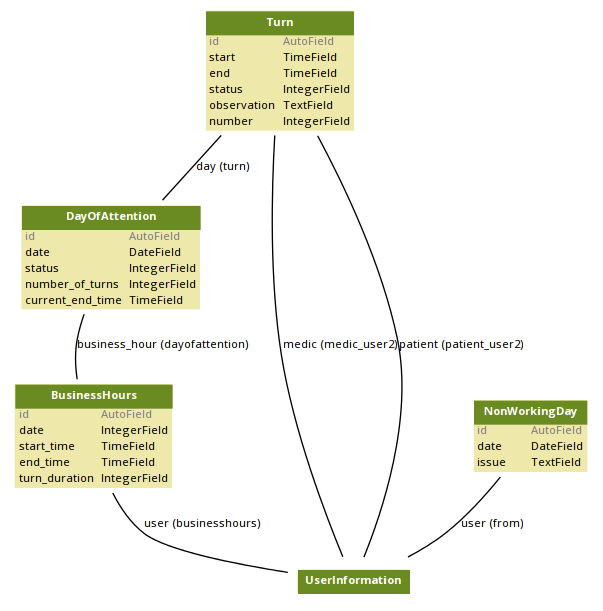
\includegraphics[scale=0.5]{resourse/gt-gt.png}
%    \caption{Vista del Panel Administracion provisto por Django}
%    \label{fig:123}
%\end{figure} 

FALTAN GRAFICOS DE AQUI


\subsubsection{Consulta Medica}


%\section{Elecci\'on de la metodolog\'ia de Programaci\'on}


\chapter{Instalacion y Configuracion}

En este Capitulo Aparte de guiarle para realizar una exitosa implementacion
Local del Servidor de Produccion se hara referencia a cada una de las
Herramientas y librerias Utilizadas.

\section{Requerimientos}

\subsection{Requerimientos de Hardware}

Cualquier equipo que cumpla con las Caracteristicas para correr Windows 7 es suficiente
en terminos de requerimientos minimos de Hardware siempre y cuando el numero de usarios
esperados no sea alto, despues el resto dependera de sus necesidades.\\[0.5cm]

\begin{itemize}
    \item Procesador x86, x64 de 1 Ghz o superior.
    \item Memoria Ram 1 GB o Superior 
\end{itemize}


\subsection{Requerimientos de Software}


\begin{itemize}
    \item Apache 2.2
    \item PosgreSQL 9.2
    \item Python 2.7.x o Python 2.6.x
    \item Django 1.3.x o Superior
    \item PGAdmin
    \item psycopg2
    \item mod\_wsgi
    \item ReportLab
    \item easy\_thumbnails
    \item django\_extensions
    \item django\_cron
\end{itemize}


\section{Apache}

Existen 2 caminos para instalar Apache La Primera Hacer una instalacion Limpia
de Apache, la 2da es cuando no se quiere trastear con tanta configuracion por lo que
opta por infraestructuras tipo WAMP, LAMP, WAPP, etc.

\subsection{Instalacion en Limpio}

Solo recomiendo este tipo de instalacion desde 0 para quienes ya poseen un conocimiento
avanzado en cuanto a manejo de servidores.

Descargamos de \url{Apache.org} la ultima version disponible, puedes utilizar el siguiente
vinculo: \url{http://www.apachehaus.com/cgi-bin/download.plx}. \\ 
Crea dos carpetas en la unidad C, la primera de nombre {\bfseries Apache} y la segunda
{\bfseries servidor}. Descomprime el archivo descargado y ejecútalo,
sigue los pasos de la instalación y de los datos que te piden solo escoge el
destino de la instalación, que será la carpeta que creaste en
{\bfseries C:\textbackslash Apache }, los otros datos déjalos de la forma
predeterminada para configurarlos más tarde.
El programa al instalarse crea un icono en el área de notificación que te
permitirá: iniciar, detener y reiniciar Apache; tienes que tener en cuenta que
cualquier cambio que hagas en el archivo de configuración no tendrá efecto
hasta que reinicies el servidor.

\subsection{Instalacion mediante WAMP, LAMP, MAMP, WAPP}

Existem una infinidad de Paquetes precompilados y configurados, con Apache, PHP, PosgreSQL o MySQL y mas.
Dichas infraestructuras suelen nombrarse como el acronomico de las herramientas que agrupan por ejemplo:\\[1cm]

\begin{itemize}
    \item {\large WAMP {\bfseries W}indows {\bfseries A}pache {\bfseries M}ySQL {\bfseries P}HP}
    \item {\large WAPP  {\bfseries W}indows {\bfseries A}pache {\bfseries P}osgreSQL {\bfseries P}HP}  
    \item {\large LAMP {\bfseries L}inux {\bfseries A}pache {\bfseries M}ySQL {\bfseries P}HP} 
    \item {\large MAMP {\bfseries M}ac OS {\bfseries A}pache {\bfseries M}ySQL {\bfseries P}HP}  
\end{itemize}


Algunas distribuciones mas usadas disponibles Para Windows son WAMP Server \url{http://www.wampserver.com/} (WAMP),
XAMPP \url{http://sourceforge.net/projects/xampp/} (WAMP + Perl), Bitnami \url{http://bitnami.com/stack/wapp} (WAPP)
solo nos resta elegir cualquiera de ellas e instalarlas, aparte de la ruta de instalacion nos pediran el usuario y
contraseña para acceder al motor de Base de Datos.

\subsection{Configuracion}

Toda la configuración para el funcionamiento de Apache se guarda en un archivo
de texto nombrado: {\bfseries httpd.conf} que se encuentra en la ruta
{\bfseries C:\textbackslash Apache \textbackslash conf } si realizamos una instalacion en limpio o
{\bfseries C:\textbackslash wamp \textbackslash bin \textbackslash  Apache \textbackslash conf } si
instalamos el paquete multiple preconfigurado no es necesario realizar este paso por lo
que lo podremos salta.\\

Al archivo {\bfseries httpd.conf} lo podemos editar en cualquier editor de texto como Notepad.

Buscamos la linea que dice

\begin{lstlisting}[style=consola, numbers=none]
    Listem LocalHost:80
\end{lstlisting}

y la Cambiamos por:

\begin{lstlisting}[style=consola, numbers=none]
    Listem 80
\end{lstlisting}

Ahora buscamos la instruccion:

\begin{lstlisting}[style=consola, numbers=none]
    DocumentRoot "C:\xxxxxxxx"
\end{lstlisting}

y la Cambiamos por:

\begin{lstlisting}[style=consola, numbers=none]
    DocumentRoot "C:\Servidor"
\end{lstlisting}

Recordar que al inicio de la instalacion creamos una Carpeta llamada Servidor en
la unidad C. Por ultimo solo nos queda reiniciar el servidor Apache e introducir
la siguiente direccion \url{http://127.0.0.1} si nos aparece una pagina
{\bfseries It's Work!} felicidades Apache esta Funcionando.


\subsection{Instalacion de PosgreSQL}

La versión de PostgreSQL que he utilizado durante el desarrollo del sistema es
la 9.2.x, quisas cuando leas esto haya salido una nueva version la cual no deberia
generar inconvenientes ademas de que es posible que el proceso de instalación
pueda variar.\\[0.2cm]
 
El primer paso es descargar el instalador de PostgreSQL para Windows,
lo puedes descargar desde el enlace siguiente
\url{http://www.postgresql.org/download/windows}, nos bajara un instalador similar
a {\bfseries postgresql-9.2.3-rc1-windows.exe} lo ejecutamos como administrador.\\[0.2cm]

Si tenemos activado el control de cuentas de usuario nos mostrará una advertencia
con el texto "¿Desea permitir que este programa realice cambios en el equipo?",
pulsaremos "Sí" para continuar con la instalación de PostgreSQL.\\[0.2cm]

Indicaremos la carpeta de instalación de PostgreSQL, donde se guardarán los
ejecutables, librerías y ficheros de configuración de PostgreSQL en mi caso el
directorio es {\bfseries C: \textbackslash PosgreSQL \textbackslash 9.2 },
Indicaremos también la carpeta donde se guardarán los datos por defecto
de PostgreSQL {\bfseries C: \textbackslash psql-data }.\\[0.2cm]

Solo nos queda introducir la contraseña para el superusuario "postgres" que
será con el que iniciemos sesión para administrar la base de datos, despues
podremos crear otros usuarios si es necesario. Ademas introduciremos el puerto
de escucha para la conexión con el servidor PostgreSQL, por defecto el 5432.\\[0.2cm]

Seleccionaremos la configuración regional y comenzara la instalacion, con esto
PosgreSQL quedara instalado. Si tenemos algún cortafuegos (firewall) deberemos
abrir el puerto 5432.

\subsection{Creacion de la Base de Datos}

Junto con la Instalacion de PosgreSQL se instala el PGAdmin III que es una Heramienta
GUI para administrar el motor de base de Datos. Iniciamos el Programa,
desplegaremos "Server Groups", dentro desplegaremos "Servidores" y dentro de
éste pulsaremos con el botón derecho del ratón sobre "PostgreSQL 9.0 (localhost:5432),
en el menú emergente seleccionaremos "Conectar".

Introduciremos la contraseña para el superusuario postgres
(la contraseña introducida en la instalación).

Pulsaremos con el botón derecho del ratón sobre "Bases de datos", seleccionaremos
"Nueva Base de Datos", en la pestaña "Propiedades" introduciremos los
siguientes datos:

\begin{itemize}
    \item Nombre: nombre de la base de datos, en nuestro caso "BDSem".
    \item Propietario: seleccionaremos el usuario creado anteriormente "posgres".
    \item Codificado: seleccionaremos UTF8.
    \item Tablespace: seleccionaremos el tablespace creado anteriormente "pg\_default".
    \item Colación: seleccionaremos "Spanish, Argentina".
    \item Tipo carácter: seleccionaremos "Spanish, Argentina".
\end{itemize}

Pulsaremos "OK" para crear la base de datos, con esto ya tendremos nuestra base
de datos aunque vacia, el resto como creacion de las Tablas correspondientes
nesesarias para el proyecto lo haremos mas adelante mediante Django.



\section{Instalacion de Python}

Para este proyecto se utilizo CPython pero no la version Oficial url{http://www.python.org}
sino la que distribuye Active State \url{http://www.activestate.com} llamada
{\bfseries Active Python} la cual provee caracteristicas adicionales a version oficial,
podremos descargar la ultima version desde \url{http://www.activestate.com/activepython/downloads}
aunque se recomienda instalar la version 2.7.x para evitar cualquier posible problema.

\subsection{Probando Python}
Para probar que la instalacion haya sido correcta abriremos la Terminal "cmd.exe"
y escribiremos:

\begin{lstlisting}[style=consola, numbers=none]
    python
\end{lstlisting} 

Si todo va bien nos debera aparecer algo similar a:

\begin{figure}[h]
    \centering
    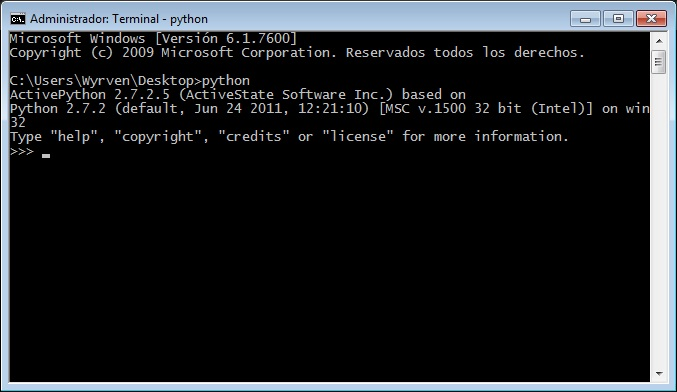
\includegraphics[scale=0.7]{resourse/consola-python.jpg}
    \caption{Ejecutando Python en la Terminal}
    \label{fig:01}
\end{figure}    

En caso contrario deberias revisar que la ruta de Python este dentro de la variable
 PATH del sistema.





%\section{Django}

Django es un framework de desarrollo web de código abierto, escrito en Python,
que respeta el paradigma conocido como {\bfseries Model Template View}. Fue desarrollado en
origen para gestionar varias páginas orientadas a noticias de la
{\bfseries World Company de Lawrence, Kansas}, y fue liberada al público bajo una licencia
BSD en julio de 2005; el framework fue nombrado en alusión al guitarrista de
jazz gitano Django Reinhardt \url{http://es.wikipedia.org/wiki/Django_Reinhardt}.

En junio del 2008 fue anunciado que la recién formada Django Software Foundation
se haría cargo de Django en el futuro.

La meta fundamental de Django es facilitar la creación de sitios web complejos.
Django pone énfasis en el re-uso, la conectividad y extensibilidad de
componentes, el desarrollo rápido y el principio No te repitas
(DRY, del inglés Don't Repeat Yourself). Python es usado en todas las partes
del framework, incluso en configuraciones, archivos, y en los modelos de datos.


\subsection{MVC}

Antes de Explicar como funciona Django empezare por una breve explicacion de
el patr\'on (MVC) Modelo Vista Controlador el cual es un patrón de arquitectura de software que
separa los datos y la lógica de negocio de una aplicación de la interfaz de
usuario y el módulo encargado de gestionar los eventos y las comunicaciones.
Para ello MVC propone la construcción de tres componentes distintos que son el
modelo, la vista y el controlador, es decir, por un lado define componentes
para la representación de la información, y por otro lado para la interacción
 del usuario. Este patrón de diseño se basa en las ideas de reutilización de
 código y la separación de conceptos, características que buscan facilitar la
 tarea de desarrollo de aplicaciones y su posterior mantenimiento.

De manera genérica, los componentes de MVC se podrían definir como sigue:

{\bfseries  El Modelo:} Es la representación de la información con la cual el sistema opera,
por lo tanto gestiona todos los accesos a dicha información, tanto consultas
como actualizaciones, implementando también los privilegios de acceso que se
hayan descrito en las especificaciones de la aplicación (lógica de negocio).
Envía a la 'vista' aquella parte de la información que en cada momento se le
solicita para que sea mostrada (típicamente a un usuario). Las peticiones de
acceso o manipulación de información llegan al 'modelo' a través del
'controlador'.

{\bfseries El Controlador: } Responde a eventos (usualmente acciones del
usuario) e invoca peticiones al 'modelo' cuando se hace alguna solicitud sobre
la información (por ejemplo, editar un documento o un registro en una base de
datos). También puede enviar comandos a su 'vista' asociada si se solicita un
cambio en la forma en que se presenta de 'modelo' (por ejemplo, desplazamiento
 o scroll por un documento o por los diferentes registros de una base de datos),
  por tanto se podría decir que el 'controlador' hace de intermediario entre
   la 'vista' y el 'modelo' actuando como Middleware
\footnote{Middleware es el software que proporciona un enlace entre aplicaciones de software
independientes. Middleware a veces se llama a la vía que conecta dos
aplicaciones y pasa los datos entre ellas. Los Middleware permiten que los
datos contenidos en una base de datos puedan ser accedidos a través de otra.
Ahorra el tiempo a los programadores.}.
   
{\bfseries La Vista: } Presenta el 'modelo' (información y lógica de negocio)
 en un formato adecuado para interactuar (usualmente la interfaz de usuario)
 por tanto requiere de dicho 'modelo' la información que debe representar como
 salida.

\begin{figure}[h]
    \centering
    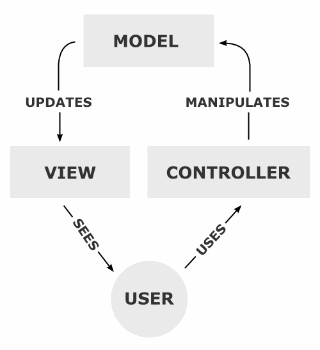
\includegraphics[scale=0.7]{resourse/MVC-Process.png}
    \caption{Diagrama del Patron MVC Modelo Vista Controlador}
    \label{fig:03}
\end{figure}    


\subsection{Django y el MVT}

Si hicieramos una clasificacion de Herramientas de desarrollo web, podriamos
clasificar a Django como parte de la tercera generacion:


\begin{figure}[h]
    \centering
    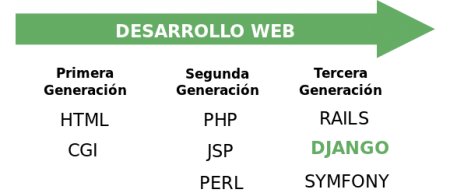
\includegraphics[scale=0.7]{resourse/desarrolloweb.png}
    \caption{Generaciones de Herramientas de Desarrollo Web}
    \label{fig:02}
\end{figure}   

Sin embargo más alla de las clasificaciones que podr\'ian existir, está el
entender como funciona realmente, al entenderlo se puede llegar a dominarlo.

Dijimos que era un framework MTV (una modificación de MVC, nada que ver con
un canal de m\'usica), esto se debe a que los desarrolladores no tuvieron la
 intención de seguir algún patron de desarrollo, sino hacer el framework lo
más funcional posible.

\begin{itemize}
    \item {\bfseries  El Modelo} en Django sigue siendo el modelo
    \item {\bfseries La Vista} en Django se llama Plantilla (Template)
    \item {\bfseries El controlador} en Django se llama Vista
\end{itemize}

Una imagen nos hará entender mejor esta relación:

\begin{figure}[h]
    \centering
    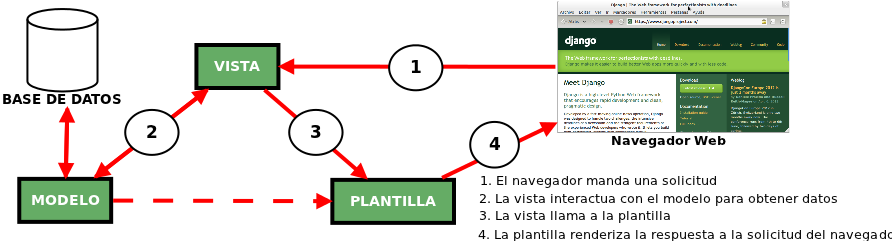
\includegraphics[scale=0.5]{resourse/esquema-mtv.png}
    \caption{El patron Modelo Vista Template de Django}
    \label{fig:04}
\end{figure}   



\subsection{El Modelo}
El modelo define los datos almacenados, se encuentra en forma de clases de
Python, las clases definidas son traducidas por Django y este genera las Tablas
necesarias para el funcionamiento del modelo dentro de la base de datos, cada
tipo de dato que debe ser almacenado se encuentra en una variable 
con ciertos parámetros, posee métodos también. Todo esto permite indicar y
controlar el comportamiento de los datos.\\[0.1cm]

Aqui un extracto del codigo mostrando como se implementa uno de los tantos
modelos con los que trabaja el Sistema\\[0.3cm]


\begin{lstlisting}[style=Python]

class Message(models.Model):
    """
        Clase Para Manejar mensajes entre usuarios
    """
    from_user = models.ForeignKey(User, related_name='from_user')
    to_user = models.ForeignKey(User, related_name='to_user')
    date = models.DateTimeField("Fecha y Hora",auto_now_add=True)
    issue = models.CharField("Asunto",max_length=125, default='')
    content = models.TextField("Cuerpo del Mensaje")
    read = models.BooleanField("Leido",default=False)


    class Meta:
        db_table = "Messages"
        verbose_name = "InboxMessage"
        verbose_name_plural = "InboxMessages"
\end{lstlisting}

\footnote{Como algunos lo notaran la variable from\_user del modelo internamente
es una relacion 1:M dentro de la base de datos.}

\footnote{La Clase interna Meta define atributos expeciales como 'db\_name' que hace
referencia a como se llamara la tabla dentro de la Bases de Datos.}

\vspace{0.1cm}

\subsection{La Vista}
La vista se presenta en forma de funciones en Python, su propósito es
determinar que datos serán visualizados, entre otras cosas más que iremos
viendo conforme avanzamos con el curso. El ORM de Django permite escribir
código Python en lugar de SQL para hacer las consultas que necesita la vista.
La vista también se encarga de tareas conocidas como el envío de correo
electrónico, la autenticación con servicios externos y la validación de
datos a través de formularios. Lo mas importante a entender con respecto a la
 vista es que no tiene nada que ver con el estilo de presentación de los
 datos, sólo se encarga de los datos, la presentación es tarea de la plantilla.\\[0.1cm]


Aqui muestro una vista sencilla que realiza una consulta base de datos que listara todos
los usuarios que sean medicos. \\[0.1cm]

\begin{lstlisting}[style=Python]
def patient_show_medics_list(request):
    """
        Muestra el listado de Medicos
    """
    mi_template = get_template('Patients/GestionTurnos/medics-list.html')
    dict = generate_base_keys(request)

    if is_patient(request.user):
        dict['medics'] = UserInformation.objects.filter( \\
                                    user__groups__name='Medico')
        html_cont = mi_template.render(Context(dict))
        return HttpResponse(html_cont)

    else:
        #si hay un usuario logueado intentanto acceder sera enviado a una
        # pagina de error
        path = request.META['PATH_INFO']
        return HttpResponseRedirect("/restricted-access%s" %path)
\end{lstlisting}

\vspace{0.1cm}

Aunque es un ejemplo sencillo podemos apreciar el potencial de Django, como vemos
no vemos ningun codigo SQL, pues bien dicho codigo SQL se ejecuta internamente
nos aleja del problema de las restriciones de la Base de Datos ya sea que usemos
PosgreSQL (como en este sistema), MySQL, SQLServer o SQLite nosotros
solo escribiremos codigo Python, El framework se encargargara de traducir esa
instrucion al motor de bases de datos correspondiente que estemos usando.\\[0.2cm]

\begin{lstlisting}[style=consola]
dict['medics'] = UserInformation.objects.filter( \\
                            user__groups__name='Medico')
\end{lstlisting}

\vspace{0.1cm}

Traducido a SQL terminariamos con algo tan orrible como esto:\\[0.1cm]

\begin{lstlisting}[style=consola]
SELECT * FROM UserInformation as Info
INNER JOIN User ON Info.username = User.username
INNER JOIN GroupsByUsers ON User.username = GroupsByUsers.username
...
\end{lstlisting}

\vspace{0.1cm}

\subsection{La Plantilla}
La plantilla es básicamente una página HTML con algunas etiquetas extras
propias de Django, en si no solamente crea contenido en HTML (también XML, CSS,
Javascript, CSV, etc).\\[0.1cm]

La plantilla recibe los datos de la vista y luego los organiza para la
presentación al navegador web. Las etiquetas que Django usa para las plantillas
permiten que sea flexible para los
diseñadores del frontend, pueden Extenderse a partir de otras plantillas incluso
tiene estructuras de datos como if, por por si es necesaria una presentación
lógica de los datos, estas estructuras
son límitadas para evitar un desorden poniendo cualquier tipo de código Python.\\[0.1cm]

Esto permite que la lógica del sistema siga permaneciendo en la vista. Aqui la
vista para Iniciar Session:\\[0.1cm]

\begin{lstlisting}[style=HTML]



<link type="text/css" rel="stylesheet" media="all"
    href="/media/css/fancy-forms.css" />
<link type="text/css" rel="stylesheet" media="all"
    href="/media/css/gradient-buttons.css" />
<link type="text/css" rel="stylesheet" media="all"
    href="/media/css/messages.css" />




<br /><br /><br />
        
            <div class="fancy-form-white" style="width: 350px;
                margin: 0 auto;">
                <h3 class="title">Inciar Session</h3><br />
                <form action="." method="POST">
                <table style="margin: 0 auto; width: 330px;" >
                <tr>
                    <td><label for="username">Usuario:</label></td>
                    <td><input type="text" name="username" value=""
                    tabindex="1" id="username"></td>
                    <td rowspan="2">
                    <input type="submit" value="Login" tabindex="3"
                    class="grad-button-blue" style="height: 50px;">
                    </td>
                </tr>
                <tr>
                    <td><label for="password">Contrase\~na:</label></td>
                    <td><input type="password" name="password" value=""
                     tabindex="2" id="password"></td>
                </tr>
                </table>
                </form>
                <br />
            </div>

            
                    <br />
                    <br />
                <div class="alert">Alerta: Error Usuario y/o Contrase\~na
                Incorrectos</div>
            

        
            <div class="alert">Alerta: Usted ya ha iniciado session con el
            usuario <strong>{{ username }}</strong></div>
            <br />
            <a href="/logout">Cerrar Session</a>
        

\end{lstlisting}

\vspace{0.1cm}

\subsection{La Configuracion de Rutas}

Django posee un mapeo de URLs que permite controlar el despliegue de las vistas,
esta configuración es conocida como URLConf. El trabajo del URLConf es leer
la URL que el usuario solicitó, encontrar la vista apropiada para la solicitud
y pasar cualquier variable que la vista necesite para completar su trabajo. El
URLConf esta construido con expresiones regulares en Python y sigue la filosofia
de Python: Explicito es mejor que implícito. Este URLConf permite que las rutas
que maneje Django seán agradables y entendibles para el usuario.\\[0.1cm]

Fragmento del archivo urls.py del Proyecto\\[0.1cm]

\begin{lstlisting}[style=HTML]
    (r'^$', base_views.index),
    (r'^index/$', base_views.index),
    (r'^login/$', base_views.login),
    (r'^logout/$', base_views.logout),
    (r'^change-password/$', base_views.change_password),
    (r'^restricted-access/$', base_views.restricted_access),
    (r'^restricted-access/(.+)/$', base_views.restricted_access),
\end{lstlisting}

\vspace{0.1cm}


\subsection{Instalar Django}

Puedes bajarte Django desde el siguiente enlace \url{https://www.djangoproject.com/download/1.3.7/tarball/}
\footnote {la version 1.3.7 no es la ultima version disponible a la hora de crear
este informe estaba por la 1.6.2 ya que Django se actualiza constantemente.}
te descargara un paquete llamado Django-1.3.7.tar.gz lo descomprimes en
algun directorio luego abres la Terminal y te posicionas sobre el directorio
donde descomprimiste y ejecutas:

\begin{lstlisting}[style=consola]
    $ python setup.py install 
\end{lstlisting}
\vspace{0.1cm}

Sino mediante el instalador de Paquetes de Python de manera mas automatica escribes
en la terminal

\begin{lstlisting}[style=consola]
     pip install django==1.3.7
\end{lstlisting}
\vspace{0.1cm}

Con esto ya tendremos instalado Django.

\section{Instalando el Resto de Las Dependencias}

Ademas de Django en el Proyecto se utilizaron otras Librerias de Python las cuales
algunas vienen instaladas y Otras Requieren ser instaladas de manera similar
a como instalamos Django.

\subsection{psycopg2}

psycopg2 es un adaptador de base de datos PostgreSQL para el lenguaje de
programación Python. psycopg2 fue escrito con el objetivo de ser muy pequeño
y rápido y estable. 

psycopg2 es diferente del otro adaptador de base de datos, ya que fue diseñado
para aplicaciones en gran medida de subprocesos múltiples que crean y destruyen
un montón de cursores y hacen que un número notable de inserciones o
actualizaciones concurrentes. psycopg2 también proporcionan operaciones
asincrónicas completos y apoyo a las bibliotecas de co-rutinas. 

Para instalar descargue el precompilado desde \url{http://www.stickpeople.com/projects/python/win-psycopg/}
Ejecutelo con permisos de administrador, nos pedira que selecionemos la version
de python con que se instalar.

\subsection{ReportLab}

ReportLab es la ultra-robusto motor de código abierto a prueba de tiempo para
la creación de documentos PDF y gráficos vectoriales personalizado. Escrito en
Python, ReportLab es rápido, flexible y una plataforma cruzada.
 
Proporciona un completo conjunto de herramientas de programación para la
creación de documentos y gráficos complejos. Ofrecemos una serie de componentes
 de forma gratuita y de código abierto, además de un paquete comercial con
características adicionales.

Para Instalar descargue el instalado desde \url{http://www.reportlab.com/software/installation/}
y proceda de manera similar a como hizo con la instalacion de psycopg2.


\subsection{easy\_thumbnails}


\subsection{django\_extensions}


\subsection{django\_cron}

Django-cron permite ejecutar código de Django de manera recurrente para el
seguimiento y ejecución de las tareas. En este caso no es Necesario Instalar
Nada, viene junto con el Codigo Fuente del Proyecto. Igualmente si tiene curiosidad
puede visitar la pagina del proyecto \url{https://github.com/Tivix/django-cron}





\chapter{Guia de Referencia}

El presente capitulo no pretende ser un completo manual de usuario de la aplicacion, 
el sistema en si es bastante intuitivo en cuanto a su funcionamiento igual aqui
se resumira un poco el funcionamiento y algunas de las diferentes sessiones de de 
la Aplicacion.

\section{Organizacion de la Aplicacion}

La aplicacion se organiza de la siguiente manera, con las diferentes sessiones
bien definidas:

\begin{itemize}
    \item 1 Menu Principal
    \item 2 Menu Secundario
    \item 3 Cuerpo de la Aplicacion
    \item 4 Informacion de Usuario
\end{itemize}

\begin{figure}[H]
    \centering
    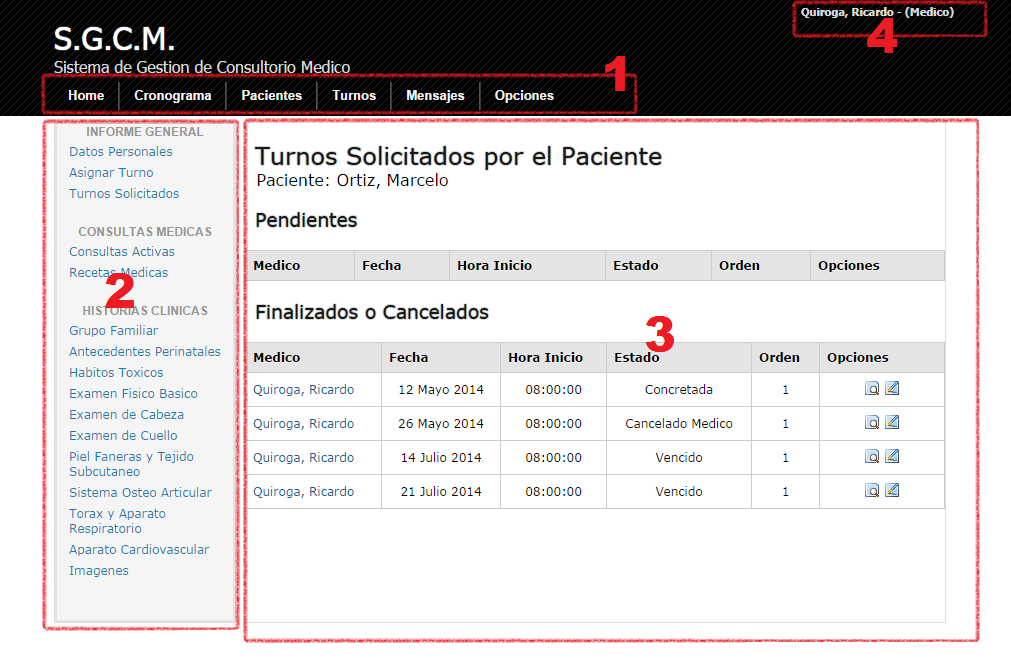
\includegraphics[scale=0.5]{resourse/organizacion.png}
    \caption{Organizacion Espacial del contenido de la aplicacion}
    \label{fig:61}
\end{figure}


\subsection{Menu Principal}

El contenido del menu principal depende del tipo de usuario que haya iniciado session
en base a ello tendra o no habilitadas diferentes funcionalidades de la aplicacion,
los unico menus comuneos son \textbf{Mensajes} y \textbf{Opciones}.


\subsection{Menu Secundario}

El menu secundario dependiendo de la vista donde se este, puede o no existir, y
su contenido dependera del las acciones que pueden ser realizadas en ella.


\subsection{Cuerpo de la Aplicacion}

Aqui se localizara el contenido principal de la vista, ya sea un formulario para
registrar alguna informacion, una lista para mostrar informacion etc.


\subsection{Informacion de Usuario}

Muesta informacion acerca de la session actual que se esta usando, tal informacion
es el nombre del usuario \footnote{nombre real, no el usename} y el tipo de usuario
que puede ser (Paciente, Medico, Administrativo,Not Login en caso de no haber
iniciado session)


\section{Panel de Usuario No Registrado}

Corresponde al panel que vera el usuario la primera ves que ingrese a la aplicacion
las funciones que se pueden hacer son restringidas y se limitan a:

\begin{itemize}
    \item \textbf{Inicio}: Ir a la pantalla de Inicio
    \item \textbf{Listado de Medicos}: Mostrar informacion basica acerca de los expecialistas
        con los que cuenta la institucion.
    \item \textbf{Registrarse}: Permite al usuario mediante una serie de pasos registrarse como paciente.
    \item \textbf{Iniciar Session}: Iniciar una session con un usuario registrado.
\end{itemize}

En cuanto la la vista \textbf{Inicio} es solo la pantalla principal de presentacion
de la aplicacion con un logo de fondo.

La vista \textbf{Listado de Medicos} puede consultarla en la session del
Panel del Paciente, ya que la unica diferencia considerable es que se agregan un
par de opciones que permiten al Paciente realizar algunas acciones a diferencia
del usuario no registrado que solo puede visualizar parte de la informacion.


\subsection{Registrarse}

Esta vista ofrece a los usuarios no registrados, un formulario donde deberan
cargar una serie de datos para registrarse como pacientes.

\begin{figure}[H]
    \centering
    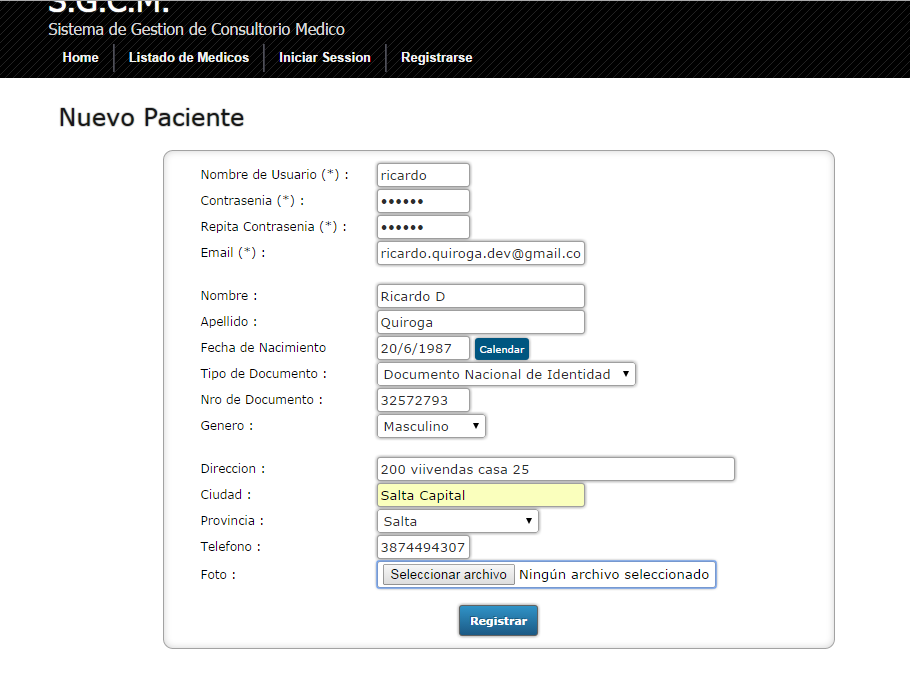
\includegraphics[scale=0.5]{resourse/registrar-paciente.png}
    \caption{Formulario Registro Paciente}
    \label{fig:62}
\end{figure}

Completado el registro y luego de enviado el formulario, si todos los datos son
correctos nos mostrara un mensaje de que el registro fue exitoso:

\begin{figure}[H]
    \centering
    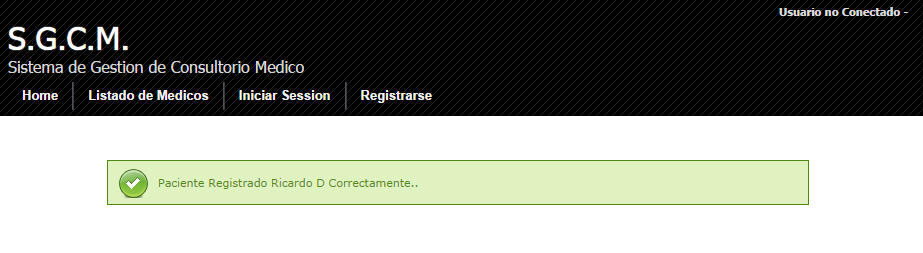
\includegraphics[scale=0.5]{resourse/registro-exito.png}
    \caption{Formulario Registro Paciente}
    \label{fig:63}
\end{figure}

Paso siguiente deveremos revisar nuestra casilla de correo donde nos aparecera
el mensaje con la direccion del formulario para activacion de usuario.
\footnote{Si se intenta iniciar session sin haber activado el usuario nos devolvera
un mensaje de error.}.

\begin{figure}[H]
    \centering
    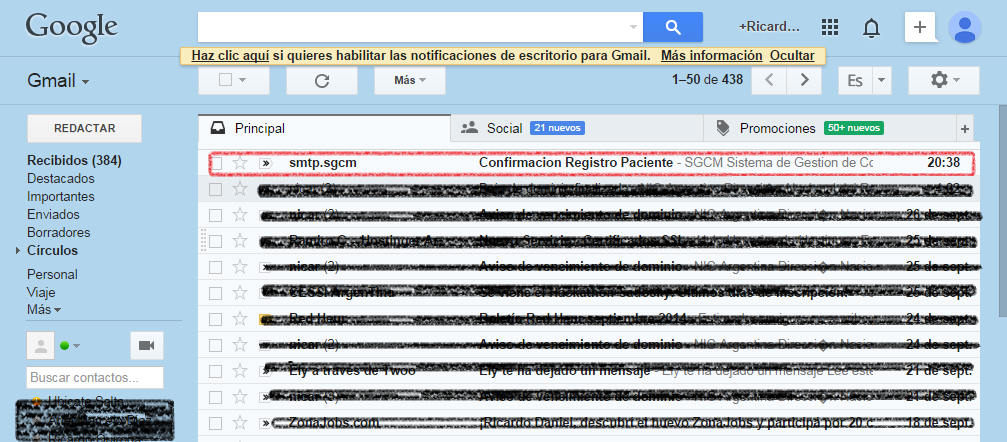
\includegraphics[scale=0.5]{resourse/correo-bandeja.png}
    \caption{Bandeja de Correo con el mensaje}
    \label{fig:64}
\end{figure}

\begin{figure}[H]
    \centering
    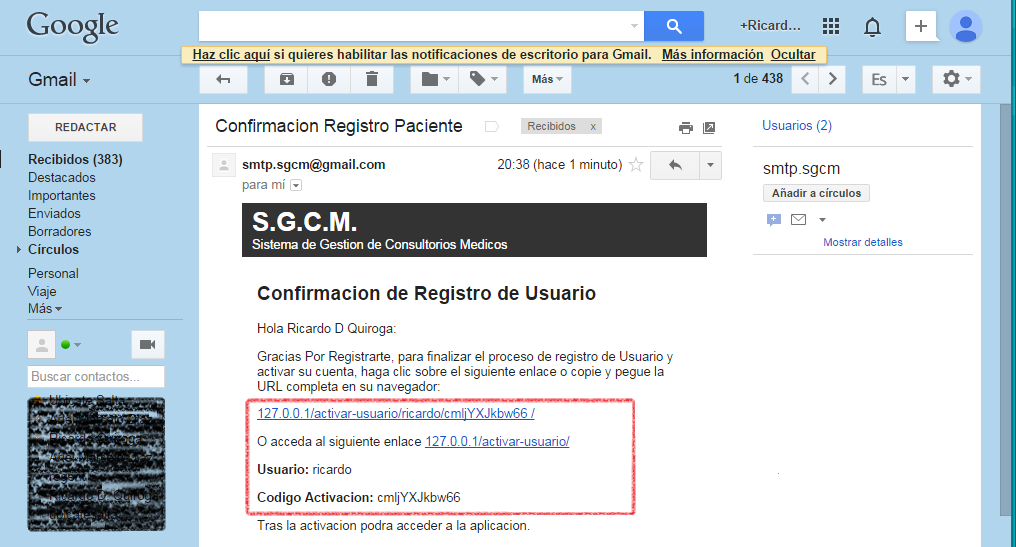
\includegraphics[scale=0.5]{resourse/correo-mensaje.png}
    \caption{Cuerpo del mensaje con la informacion de activacion de usuario}
    \label{fig:65}
\end{figure}

\begin{figure}[H]
    \centering
    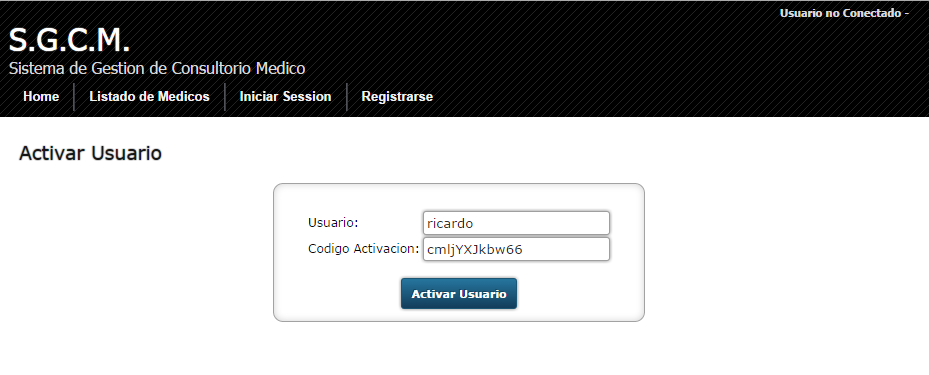
\includegraphics[scale=0.5]{resourse/usuario-activar.png}
    \caption{Formulario de Activacion de usuario}
    \label{fig:66}
\end{figure}

Luego de estos pasos el usuario estara registrado y activado, solo faltaria
iniciar session para poder empezar a operar como paciente.

\subsection{Iniciar Session}

La vista de inicio de session no es nada de otro mundo, solo es un simple
formulario donde debes introducir el usuario y contraseña validos para poder
iniciar session.


\section{Panel de Usuario Paciente}

Corresponde al panel de funciones al que tendran acceso los usuarios, pacientes
sigue siendo limitado pero ya se pueden hacer algunas cosas como solicitar
turnos y realizar consultas medicas rapidas a un expecialista, se organiza en:

\begin{itemize}
    \item \textbf{Inicio}: Ir a la pantalla de Inicio
    \item \textbf{Listado de Medicos}: Mostrar informacion  acerca de los expecialistas.
    \item \textbf{Mensajes}: Casilla de Mensajes Internos.
    \item \textbf{Mis Turnos}: Informacion acerca del estado de los turnos del usuario.
    \item \textbf{Opciones}: Panel de Opciones
\end{itemize}


\subsection{Listado de Medicos}

Vista que permite seleccionar entre el listado de expecialistas que componen el
cuerpo medico de la intitucion consultar informacion, realizar una consulta rapidas
y solicitar turno.

\begin{figure}[H]
    \centering
    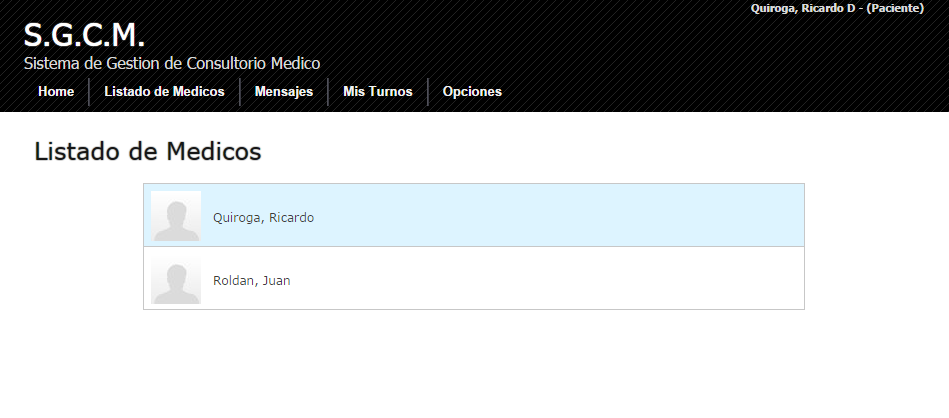
\includegraphics[scale=0.5]{resourse/listado-medico.png}
    \caption{Listado de Medicos}
    \label{fig:67}
\end{figure}

\begin{figure}[H]
    \centering
    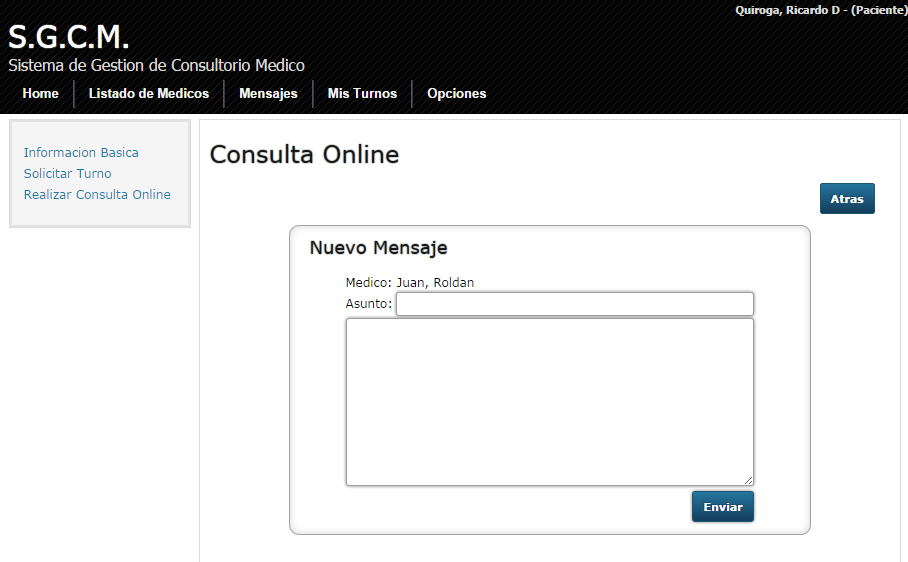
\includegraphics[scale=0.5]{resourse/consulta-online.png}
    \caption{Formulario de Consulta Online}
    \label{fig:68}
\end{figure}

\begin{figure}[H]
    \centering
    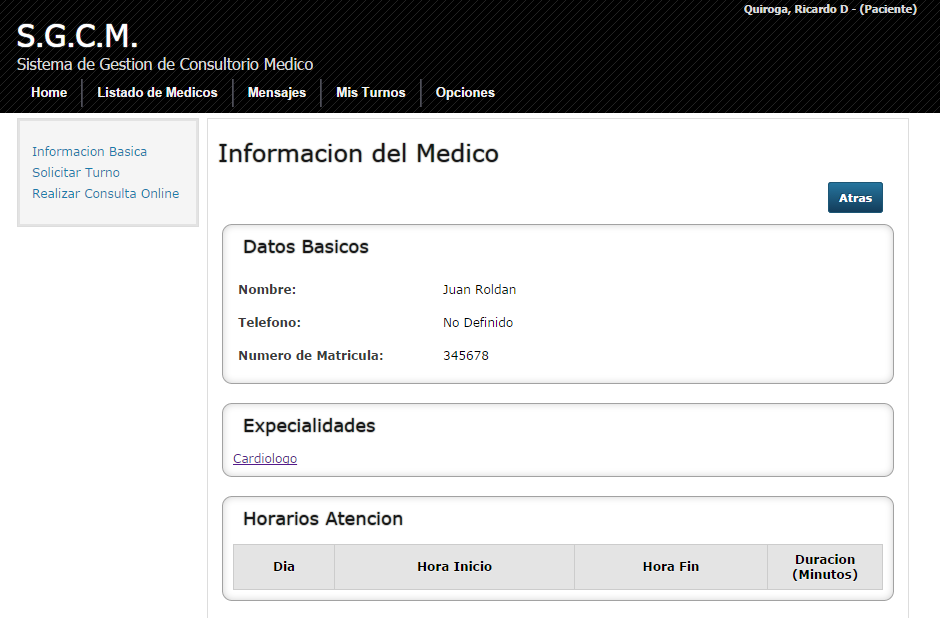
\includegraphics[scale=0.5]{resourse/medico-mostrar.png}
    \caption{Mostrar Datos del Medico}
    \label{fig:69}
\end{figure}

La vista de Asignacion de turno son similares, entre si no varian mucho por lo que
se explicara en la parte del panel de Medico.


\subsection{Mensajes}

Como ya se menciono esto es una session comun a todas los usuarios, se trata de un
conjunto de vista donde funciona el sistema de mensajeria interna entre los usuarios
de la aplicacion, su funcion esta reducida en cuanto al usuario paciente ya que
este solo puede visualizar y responder los mensajes que se le envian, para enviar
un mensaje a un profecional se realiza mediante la opcion de Realizar Consulta
Online, por lo que solo puede enviar mensaje a los expecialistas, las Opciones
disponible son:

\begin{itemize}
    \item \textbf{Redactar}: Escribir un Nuevo Mensaje
    \item \textbf{Recibidos}: Bandeja de Entrada
    \item \textbf{Enviado}: Bandeja de Salida
\end{itemize}

Algunas de las cuales pueden ser apreciadas en las siguientes capturas:

\begin{figure}[H]
    \centering
    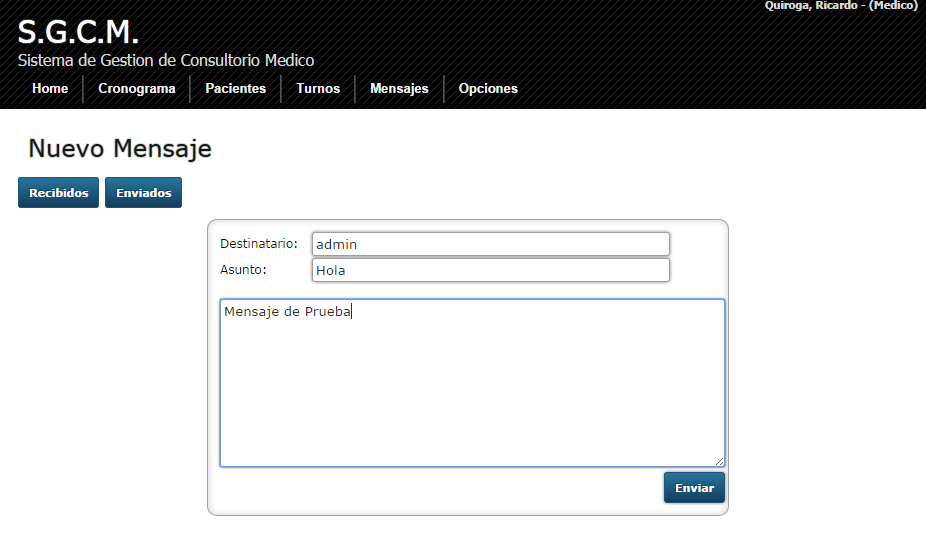
\includegraphics[scale=0.5]{resourse/mensaje-redactar.png}
    \caption{Redactar un Mensaje}
    \label{fig:610}
\end{figure}

\begin{figure}[H]
    \centering
    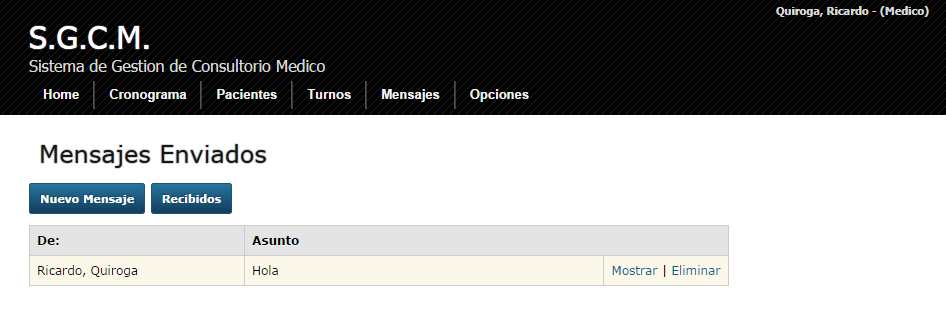
\includegraphics[scale=0.5]{resourse/mensaje-recibidos.png}
    \caption{Bandeja de Entrada}
    \label{fig:611}
\end{figure}

\begin{figure}[H]
    \centering
    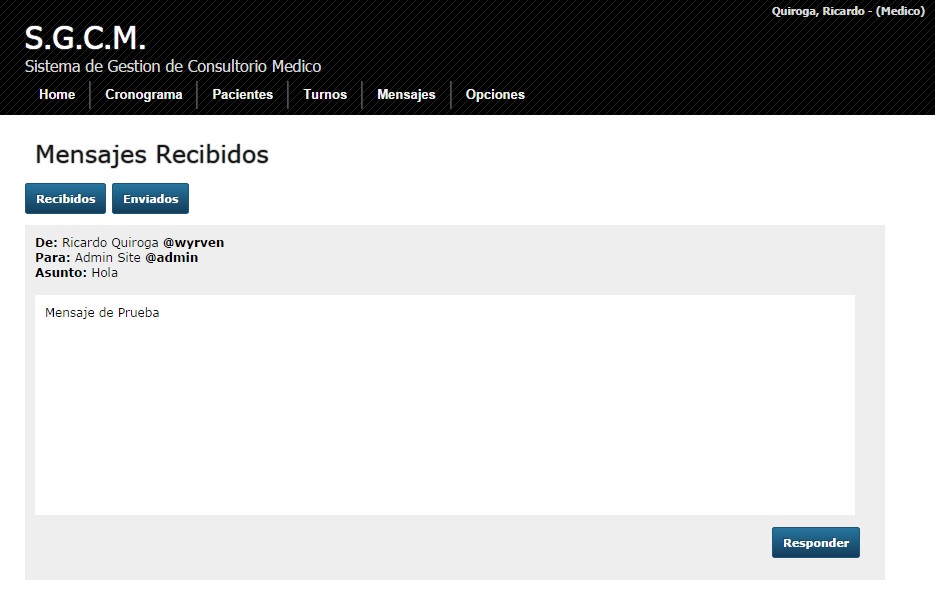
\includegraphics[scale=0.5]{resourse/mensaje-mostrar.png}
    \caption{Mostrar Mensaje}
    \label{fig:612}
\end{figure}

\subsection{Opciones}
Otro menu comun a todo los usuarios permite la administracion de los datos e
informacion del mismo, dentro de las funciones que permite este menu se encuentra:

\begin{itemize}
    \item \textbf{Mis Datos}: Mostrar/Modificar Datos personales
    \item \textbf{Camibar Contrase\~na}: Formulario para cambio de Contrase\~na
    \item \textbf{Cerrar Session}: Cerrar Session, despedirse del sistema.
\end{itemize}


\section{Panel de Usuario Administrativo}

Corresponde al panel de funciones al que tendran acceso los usuarios
Administrativos 

\begin{itemize}
    \item \textbf{Inicio}: Ir a la pantalla de Inicio
    \item \textbf{Pacientes}: Administrar Usuarios Pacientes
    \item \textbf{Medicos}: Administrar Usuarios Medicos
    \item \textbf{Administrativos}: Administrar Usuarios Administrativos
    \item \textbf{Expecialidades}: Administrar Expecialidades Medicas
    \item \textbf{Mensajes}: Casilla de Mensajes Internos.
    \item \textbf{Opciones}: Panel de Opciones
\end{itemize}


\subsection{Pacientes, Medicos, Administrativos}

Los tres conjuntos de vistas comparten muchas caracteristicas similares por lo
que se explican en conjunto y solo se mencionaran algunas de sus diferencias,
cada sub menu se enlista de acuerdo a los tipos de usuarios que se desea
administrar, permitiendo segun el sub menu la posibilidad de crear un tipo de
usuario especifico \footnote{Los Usuarios registrados por el Administrador o el
Medico no requieren activacion como los usuarios creados por usuarios no
registrados.} Buscar un usuario, modifar sus datos.


\begin{figure}[H]
    \centering
    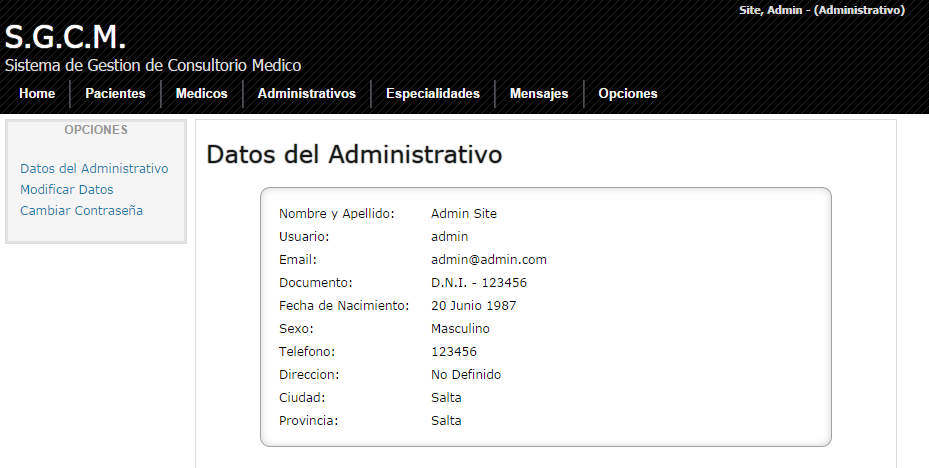
\includegraphics[scale=0.5]{resourse/datos-admin.png}
    \caption{Mostrar Administrativo}
    \label{fig:615}
\end{figure}

\begin{figure}[H]
    \centering
    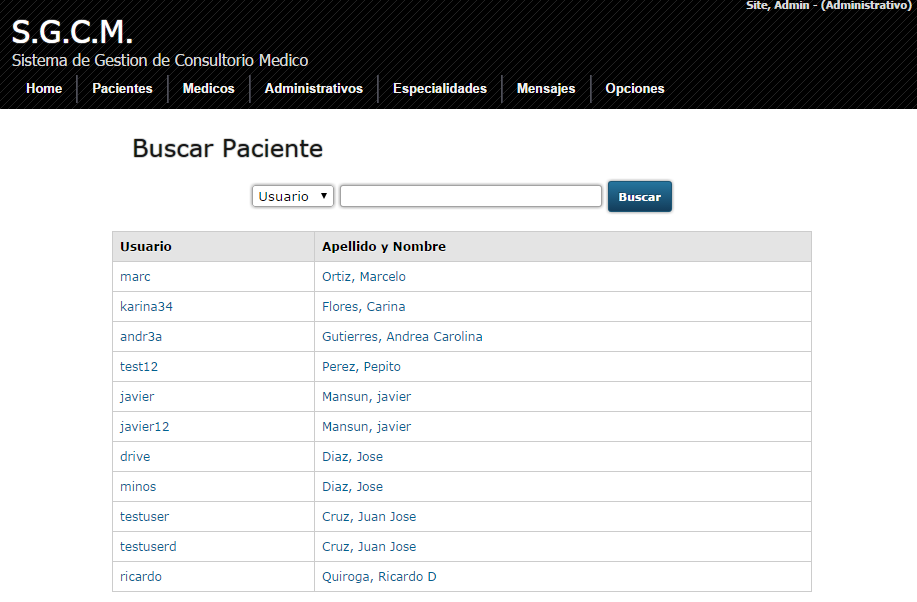
\includegraphics[scale=0.5]{resourse/listado-paciente.png}
    \caption{Vista para busqueda de usuario, en este caso usuarios Pacientes}
    \label{fig:616}
\end{figure}

En el caso de los usuarios medicos ademas puede consultar y modificar el estado
de los turnos que les fueron solicitados, definirles expecialidades
correspondiente.

\begin{figure}[H]
    \centering
    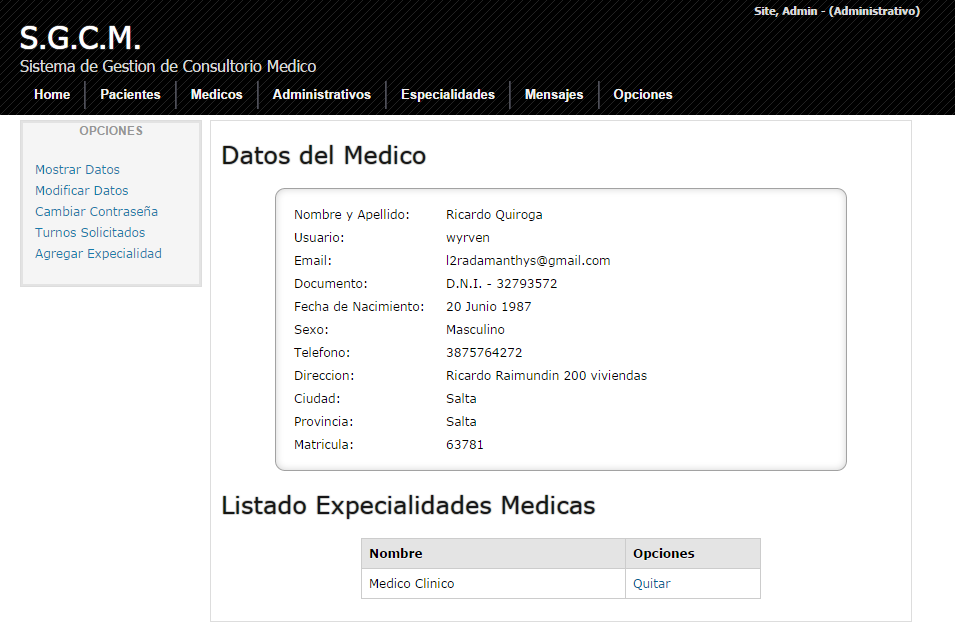
\includegraphics[scale=0.5]{resourse/datos-medico-a.png}
    \caption{Mostrar Medico}
    \label{fig:614}
\end{figure}


\begin{figure}[H]
    \centering
    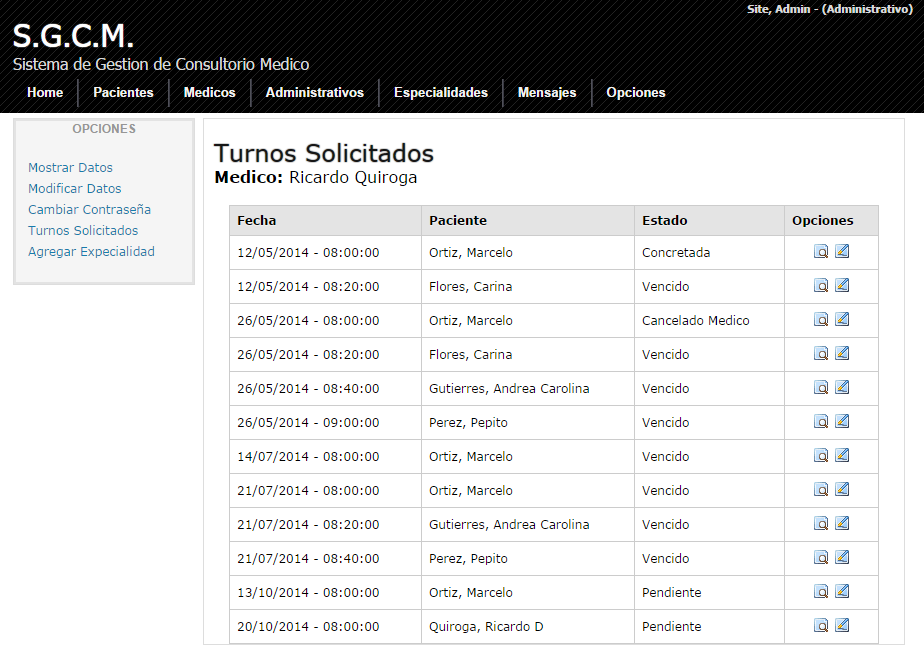
\includegraphics[scale=0.5]{resourse/turnos-sol-medico.png}
    \caption{Vista Listado Turnos Solicitados al Medico.}
    \label{fig:617}
\end{figure}


En los pacientes ademas puede asignar un turno a los mismo, cancelar un turno
solicitado por el mismo, mostrar informacion e impribir comprobante
correspondiente.

\begin{figure}[H]
    \centering
    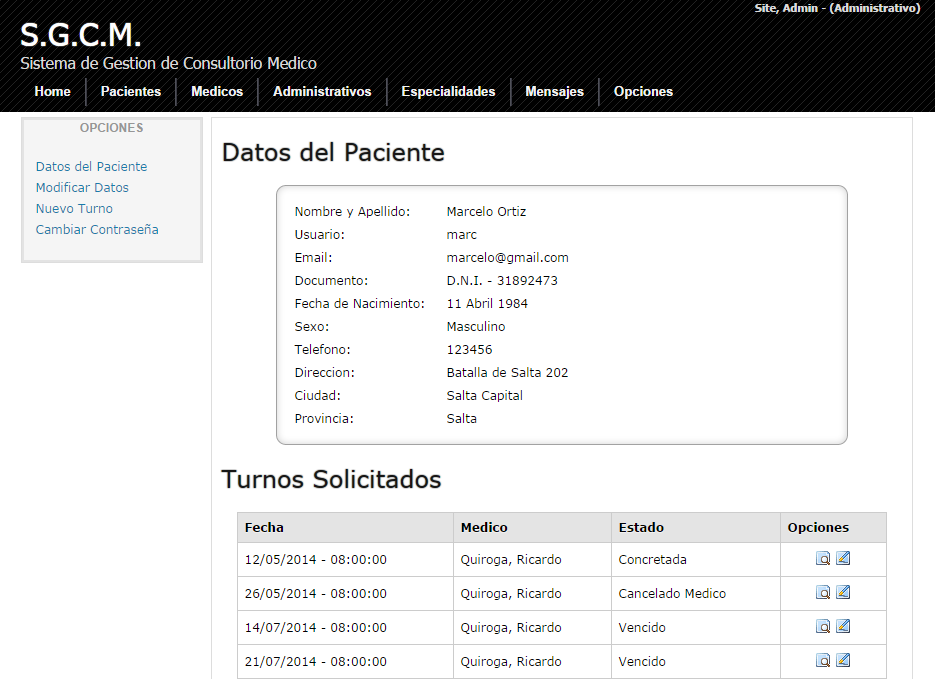
\includegraphics[scale=0.5]{resourse/datos-paciente-a.png}
    \caption{Mostrar Paciente}
    \label{fig:613}
\end{figure}



\section{Panel de Usuario Medicos}

Corresponde al panel de funciones al que tendran acceso los usuarios medicos 
aunque comparte funcionalidades en comun con los otros paneles, presenta vistas
esclusivas para el uso por parte de los medicos.

\begin{itemize}
    \item \textbf{Inicio}: Ir a la pantalla de Inicio
    \item \textbf{Cronograma}: 
    \item \textbf{Pacientes}:
    \item \textbf{Turnos}: 
    \item \textbf{Mensajes}: Casilla de Mensajes Internos.
    \item \textbf{Opciones}: Panel de Opciones
\end{itemize}

\subsection{Cronograma}

La funcionalidad de esta vista es permitir un acceso rapido a la funciones comunes,
mostrar los mensajes sin leer, y los turnos solicitados para la fecha.

\begin{figure}[H]
    \centering
    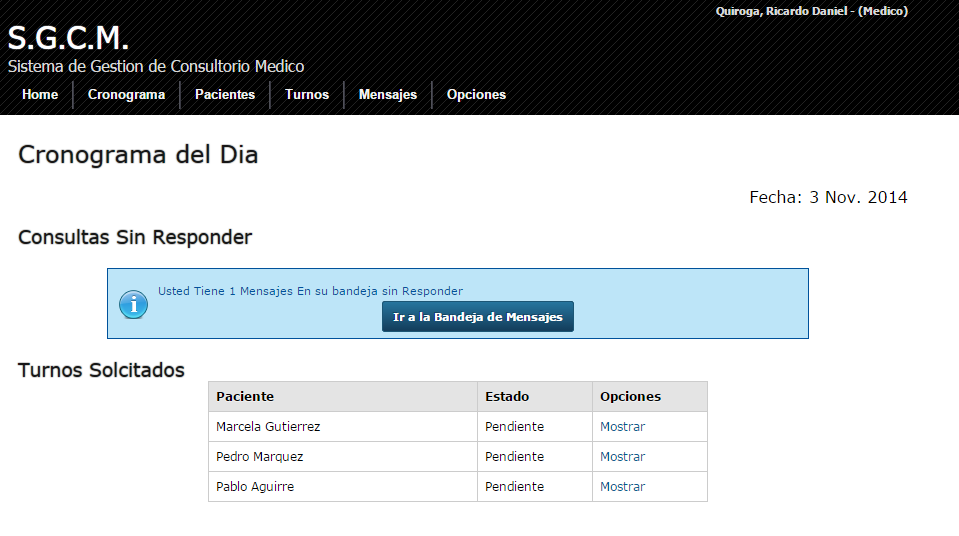
\includegraphics[scale=0.5]{resourse/cronograma.png}
    \caption{Vista del Cronograma}
    \label{fig:614}
\end{figure}


\subsection{Pacientes}

La coleccion de vistas correspondientes a los pacientes son similares a las vistas
que presenta el rol administrativo, como se menciono antes el medico tambien puede
registrar nuevos pacientes, lo que diferencia a las vistas de medico correspondiente
a esta secion es que ahora muestra un menu mas amplio de opciones en comparacion 
a la del administrador, se habilita el submenu para administrar lo referente a la
historia clinica del paciente.

\begin{figure}[H]
    \centering
    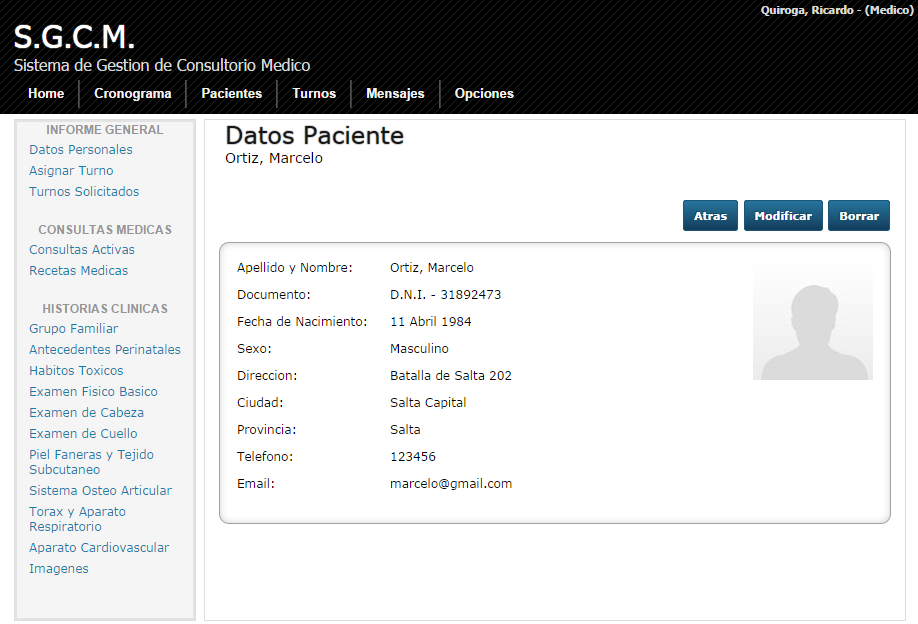
\includegraphics[scale=0.5]{resourse/datos-paciente-m.png}
    \caption{Mostrar Paciente}
    \label{fig:615}
\end{figure}

la Primera parte corresponde al registro de informacion relevante obtenida durante
la consultas medicas y prescripciones medicas \footnote{Lo que comunmente se 
conoce como receta medica.} ademas de generar el comprobante para el paciente.

\begin{figure}[H]
    \centering
    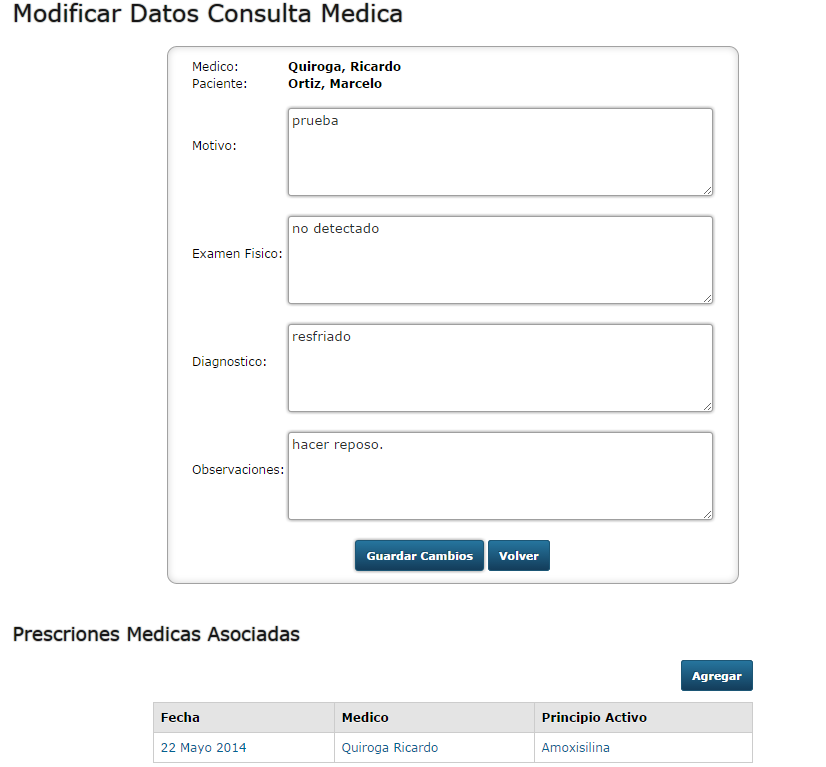
\includegraphics[scale=0.5]{resourse/consulta-medica.png}
    \caption{Consulta Medica}
    \label{fig:616}
\end{figure}

\begin{figure}[H]
    \centering
    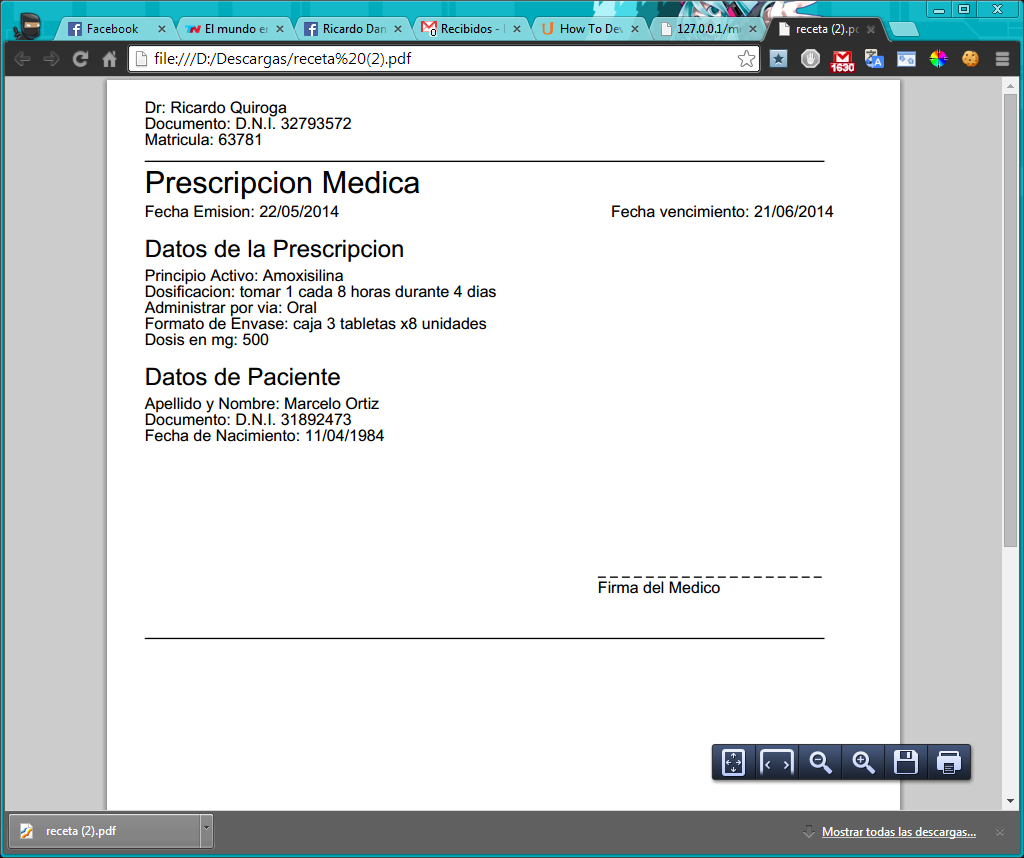
\includegraphics[scale=0.3]{resourse/receta.png}
    \caption{Imprimir Receta o Prescripcion Medica}
    \label{fig:617}
\end{figure}

En cuanto a los estudios clinicos que se registran en la historia clinica, por 
lo general al seleccionarlo puede que se visualize: 


la informacion del examen unicamente, con la opcion de modificacion si este es 
unico, por ejemplo el caso de registro de antecedentes perinatales.

\begin{figure}[H]
    \centering
    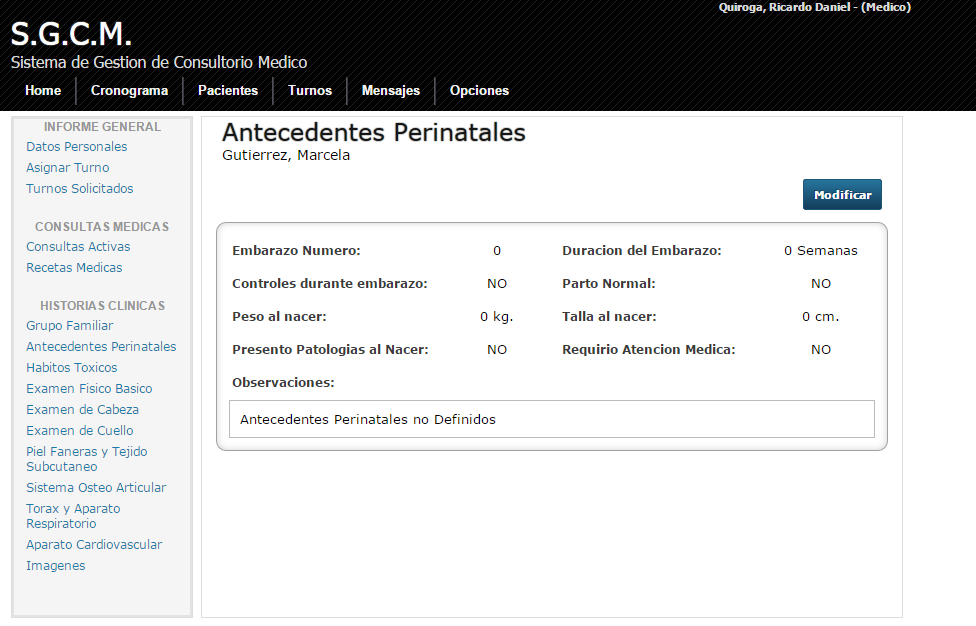
\includegraphics[scale=0.5]{resourse/modificar-perinatales.png}
    \caption{Examen Unico}
    \label{fig:618}
\end{figure}

O tambien muestre un listado con los examenes realizados donde se debera selecionar el 
examen especifico que se desea consultar, o registrar un nuevo examen en caso 
de requerirlo, como por ejemplo es el caso del examen fisico ya que al paciente 
pueden realizale durante su vida varios examenes de este tipo.

\begin{figure}[H]
    \centering
    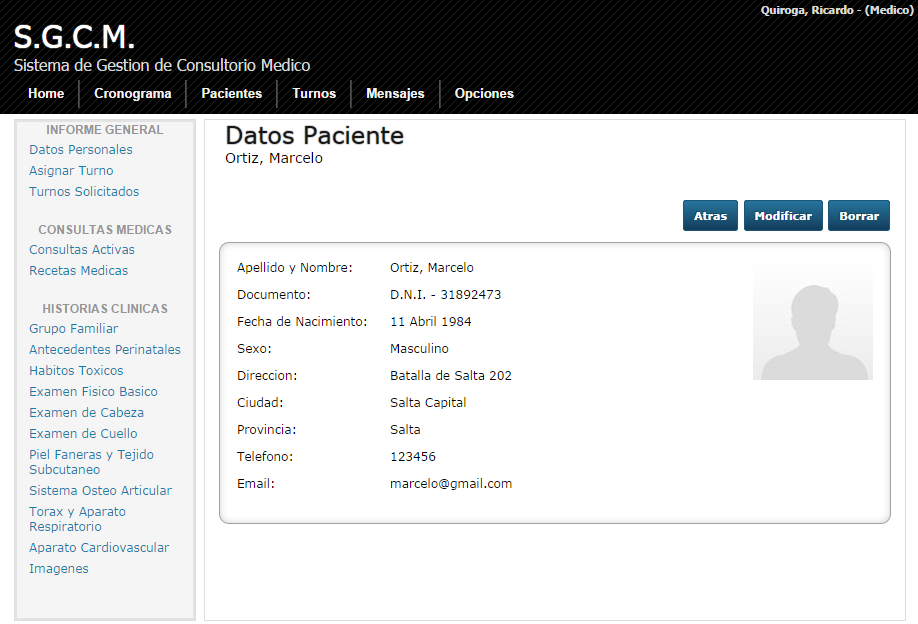
\includegraphics[scale=0.5]{resourse/datos-paciente-m.png}
    \caption{Listado de Examenes Fisicos}
    \label{fig:619}
\end{figure}

\begin{figure}[H]
    \centering
    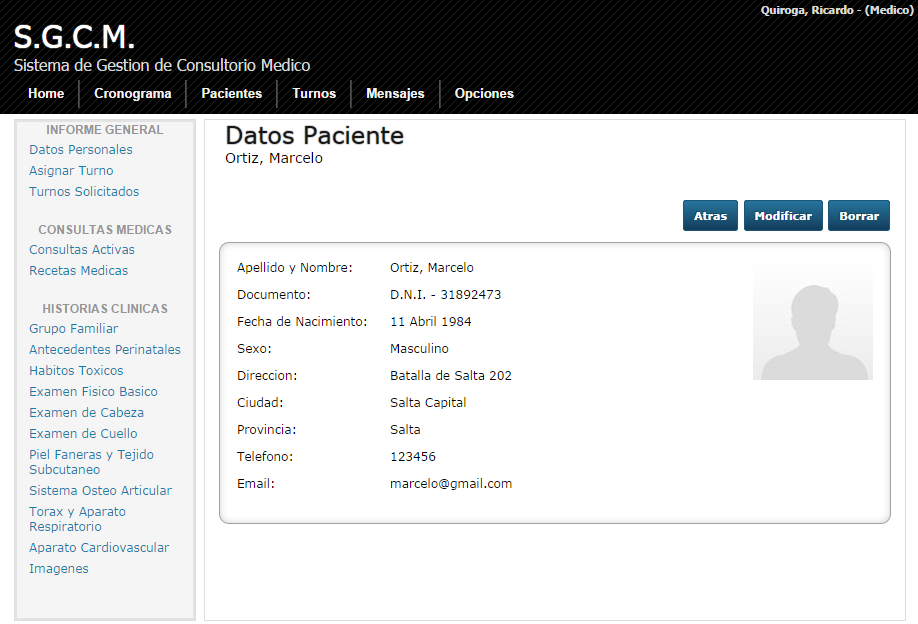
\includegraphics[scale=0.5]{resourse/datos-paciente-m.png}
    \caption{Nuevo Examen Fisico}
    \label{fig:618}
\end{figure}


\chapter{Conclusion y Mejoras}


\section{Resultado}

El Sistemas de Gestión de Consultorios Medico proporciona soporte para Gestión de Turnos para pacientes y médicos proveyendo una nueva manera de mejorar la comunicación entre el paciente y el médico atraves de Internet, Permite administrar las Historias Clínicas dejando de depender de archivos físicos y con la posibilidad de almacenar los mismos en la nube.\\[0.1cm]

Considero que se alcanzaron casi todos los objetivos planteados y otros no planteados en la etapa inicial.


\subsection{Ventajas Percibidas}

Las Ventajas y Desventajas en lo que respeta al sistema fueron expuestas en el \textit{Capítulo IV} cuando se realizo una comparación con el actual funcionamiento de la mayoría de las instituciones, aquí se analizan las relacionadas a las herramientas que se utilizaron en su desarrollo.

\begin{itemize}
    \item La primera ventaja que encontré fue la velocidad de desarrollo comparando con otras herramientas aunque Python no es un 4GL sino un 3GL la facilidad de entendimiento de su sintaxis hace que el código
        sea fácilmente entendible y legible lo que permite un mantenimiento sencillo, el código en Python se asemeja mucho a lo que hacemos cuando escribimos un algoritmo en el papel por lo que la curva de aprendizaje si ya manejas algún lenguaje es mínima.

    \item Django y el Modelo de desarrollo MVC (Modelo Vista Controlador) aportaron otro extra a la velocidad de desarrollo del sistema ya que  solo con un par de líneas era capaz de crear vistas fácilmente adaptables, además de la característica de poder heredar plantillas por lo que en caso que quisiera realizar un cambio en el diseño de la plantilla solo requería cambiar la plantilla maestra o base sin necesidad de estar modificando una por una todas las plantillas, ni hablar si el código hubiese estado mesclado con el HTML como ocurre       aveces con PHP por ejemplo.

    \item Otra característica interesante de Django que me ahorro sufrimiento fue la definición de Modelos, cuando trabajas con Django no hace falta conocer el motor de Base de Datos y su sintaxis, no te debes preocupar por aprender cómo realizar tal o cual consulta, dejas de pelear con los JOIN de SQL y demás, solo te dedicas a aprender a manejar el Object Relational Model o ORM que forma parte de Django el cual es         sencillo de aprender.

    \item Aunque no está relacionado en si con el desarrollo de manera explícita agradezco haber conocido sitios como url{http://www.stackoverflow.com} que es un sitio colaborativo donde podes hacer preguntas y/o responderlas sobre cuestiones de programación, instalaciones, errores, etc. Fue una gran ayuda ya que pude solucionar gracias a eso muchas de las dificultades y entender el problema de las mismas de manera rápida.

    \item Aprender a usar un sistema de control de versiones para el código fuente como GIT de mi proyecto fue de gran utilidad ya que el desarrollo de esta aplicación no fue de manera continua sino que variada durante todo el tiempo de desarrollo.
\end{itemize}


\subsection{Desventajas Percibidas}

No todo el desarrollo fue como se esperaba, surgieron una serie de inconvenientes o limitaciones relacionadas con la herramienta.

\begin{itemize}
    \item Hacer Deploy \footnote{Implementar un servidor de producción con Apache, Python, Django y PosgreSQl, mod\_wsgi} con la herramienta no es tan fácil como cuando instalas LAMP, pierdes mucho tiempo intentando configurar el servidor, la documentación existente sobre la misma es muy poca y normalmente incompleta.

    \item En su mayoría la documentación sobre las librerías y demás herramientas se encuentra escrita en ingles, no lo consideraría en si una desventaja pero lo menciono en este apartado por mi bajo nivel en lo que respecta a lectura y comprensión de texto en ingles.
\end{itemize}


\section{Futuras Mejoras}

El sistema podría evolucionar de varias maneras, al ser un sistema diseñado mediante plantillas la principal evolución del mismo es que se podría adaptar las interfaces a los navegadores de los dispositivos móviles inteligentes mediante un diseño responsive. \\[0.1cm]

Otra mejora común al sistema, seria que pueda integrarse con otros estudios como poder registrar análisis de laboratorio, odontograma, integración con  el sistema vademécum para que sea más sencillo elaborar una receta médica,  y la posibilidad de importar y/o exportar la historia clínica a formatos conocidos como archivos PDF para permitir ser exportado a papel.


\addcontentsline{toc}{chapter}{Glosario}
{\Huge \textbf{Glosario}}
\\[0.5cm]

Glosario de Terminos poco comunes utilizados en este Informe.
\\[0.1cm]

{\LARGE \textbf{A}}\\[0.1cm]

\textbf{Antecedentes Perinatales}: Informacion referente a la atencion durante 
el embarazo y parto.\\[0.1cm]

\textbf{Aplicacion:} Durante el informe se utilizo el nombre Aplicacion o Sistema
indistintamente para referirse al sistema en cual se basa el presente informe.
\\[0.1cm]

\textbf{Aplicacion Informatica:} En informatica, una aplicacion es un tipo de programa 
informatico dise\~nado como herramienta para permitir a un usuario realizar uno o
diversos tipos de trabajos. Esto lo diferencia principalmente de otros tipos de
programas como los sistemas operativos, las utilidades (que realizan tareas de 
mantenimiento o de uso general), y los lenguajes de programacion (con el cual se 
crean los programas informaticos).
\\[0.5cm]

{\LARGE \textbf{B}}
\\[0.1cm]
\textbf{Baterias Incluidas:} El termino hace referencia al tama\~no de la biblioteca
estandar (conjunto de modulos y librerias con que cuenta Python por defecto) ya que
la instalacion basica incluye librerias para casi todos tipo de tareas las cuales
por ende pueden ser extendidas.
\\[0.5cm]

{\LARGE \textbf{C}}
\\[0.1cm]
\textbf{Consulta Medica:} Se refiere a la cita que el paciente tiene con el expecialista.
\\[0.5cm]

{\LARGE \textbf{D}}
\\[0.1cm]
\textbf{DER:} 
\\[0.1cm]
\textbf{Deploy:}
\\[0.5cm]

{\LARGE \textbf{E}}
\\[0.1cm]
\textbf{Expecialista}: En este informe usamos el termino expecialista para referirnos
a los medicos.
\\[0.5cm]

{\LARGE \textbf{H}}
\\[0.1cm]
\textbf{Historia Clinica}
\\[0.5cm]

{\LARGE \textbf{M}}
\\[0.1cm]
\textbf{MVC:}
\\[0.5cm]

{\LARGE \textbf{N}}
\\[0.1cm]
\textbf{No Pythonico:} 
es lo contrario de Pythonico. Osea codigo fuente es ofuscado o tiene
problemas de legibilidad, es un termino de programacion. 
\\[0.1cm]
\textbf{NoSQL:}
En inform�tica, NoSQL (a veces llamado "no s�lo SQL") es una amplia clase de sistemas
de gesti�n de bases de datos que difieren del modelo cl�sico del sistema de gesti�n de
bases de datos relacionales (RDBMS) en aspectos importantes, el m�s destacado es que no 
usan SQL como el principal lenguaje de consultas. Los datos almacenados no requieren
estructuras fijas como tablas, normalmente no soportan operaciones JOIN, ni garantizan 
completamente ACID (atomicidad, consistencia, aislamiento y durabilidad), y habitualmente 
escalan bien horizontalmente.
\\
Por lo general, los investigadores acad�micos se refieren a este tipo de bases de 
datos como almacenamiento estructurado, t�rmino que abarca tambi�n las bases de datos 
relacionales cl�sicas. A menudo, las bases de datos NoSQL se clasifican seg�n su forma 
de almacenar los datos, y comprenden categor�as como clave-valor, las implementaciones
de BigTable, bases de datos documentales, y Bases de datos orientadas a grafos.
\\[0.5cm]

{\LARGE \textbf{O}}
\\[0.1cm]
\textbf{Ofuscado:} 
La ofuscaci�n se refiere a encubrir el significado de una comunicaci�n haci�ndola m�s 
confusa y complicada de interpretar. En computaci�n, la ofuscaci�n se refiere al acto 
deliberado de realizar un cambio no destructivo, ya sea en el c�digo fuente de un programa
inform�tico o c�digo m�quina cuando el programa est� en forma compilada o binaria, con 
el fin de que no sea f�cil de entender o leer.
\\[0.5cm]

{\LARGE \textbf{P}}
\\[0.1cm]
\textbf{Prescripcion Medica}
\\[0.1cm]
\textbf{Pythonico}
\\[0.5cm]

{\LARGE \textbf{S}}
\\[0.1cm]
\textbf{SQL}
\\[0.1cm]
\textbf{Sistema}
\\[0.1cm]
\textbf{Stack}
\\[0.1cm]
\textbf{Super Usuario}
\\[0.5cm]

{\LARGE \textbf{U}}
\\[0.1cm]
\textbf{UML}
\\[0.5cm]

{\LARGE \textbf{Z}}
\\[0.1cm]
\textbf{Zen de Python} Los usuarios de Python se refieren a menudo a la Filosof�a Python
que es bastante analoga a la filosof�a de Unix. El codigo que sigue los principios de
Python de legibilidad y transparencia se dice que es "pythonico". Contrariamente, el
c�digo opaco u ofuscado es bautizado como "no pythonico" ("unpythonic" en ingl�s). 
Estos principios fueron famosamente descritos por el desarrollador de Python Tim 
Peters en El Zen de Python.
\\[0.5cm]


%\part*{\addcontentsline{toc}{part}{Apéndices}Apéndices}

% Adjustments headers
%\fancyhead[RO]{\leftmark}
%\fancyhead[EL]{\emph{Apéndice \thechapter}}

%%%%%%%%%%%%%
%\appendix
%%%%%%%%%%%%%%
%\ include{software}
%\ include{publicaciones}

\begin{thebibliography}{X}

    \bibitem{Apache} \textsc{Wikipedia} \textit{Servidor HTTP Apache} 
        http://es.wikipedia.org/wiki/Servidor\_HTTP\_Apache 

    \bibitem{ApacheUbuntu} \textit{Servidor Apache en Ubuntu} 
        http://kuyne.blogspot.com.ar/2013/03/servidor-apache-en-ubuntu-instalacion-y.html     

    \bibitem{ApacheWin} \textit{Servidor Apache en Windows} 
        http://norfipc.com/internet/instalar-servidor-apache.html

    \bibitem{MVC} \textsc{Wikipedia} \textit{El Modelo Vista Controlador}
        http://es.wikipedia.org/wiki/Modelo\_Vista\_Controlador

    \bibitem{Presc} \textsc{Rogelio León López, Bárbara Gallego Machado y José Díaz Novás} \textit{Formato recomendable para llenar la hoja de remisión médica de un paciente} 
        http://bvs.sld.cu/revistas/mgi/vol22\_2\_06/mgi10206.htm 

    \bibitem{ConWeb} \textsc{Sistema Consultorio Web} \textit{Registro Consulta}
        https://www.consultorioweb.com/intranet/doctor/pacienteConsultas.aspx
    
    \bibitem{PracHisClin} \textsc{PRACTICA FINAL OBLIGATORIA: INTERNADO ROTATORIO Y PASANTIA RURAL OBLIGATORIA} \textit{Modelo Historia Clinica} 
        http://www.med.unne.edu.ar/internado/his\_cli.pdf
    
    \bibitem{ModHistClin} \textsc{Any Flowers} \textit{Modelo Historia Clinica}
        http://www.slideshare.net/AnyFlowers/ejemplo-historia-clinica
    
    \bibitem{BiocomHistCLin} \textsc{Biocom} \textit{Formato de Historia Clinica}
        http://www.biocom.com/informatica\_medica/historia\_5\_examen\_fisico.html
    
    \bibitem{ExamReg} \textsc{Infomed Red de Salud de Cuba} \textit{Examen Fisico Regional} 
        http://www.sld.cu/galerias/pdf/sitios/pdguanabo/cap04.pdf
    
    \bibitem{ProbAudit} \textsc{ESMAS} \textit{Problemas Auditivos Comunes}
        http://www.esmas.com/salud/enfermedades/notransmisibles/368755.html
    
    \bibitem{PerdAudi} \textsc{Wikipedia} \textit{Perdida de Audicion}
        http://es.wikipedia.org/wiki/P\%C3\%A9rdida\_de\_audici\%C3\%B3n

    \bibitem{Rinolo} \textsc{Hernado Vargas Vásquez} \textit{Rinologia}
        http://sisbib.unmsm.edu.pe/BibVirtualdata/libros/Medicina/cirugia/Tomo\_V/archivos\%20PDF/7Rinologia.pdf
    
    \bibitem{Labio} \textsc{Wikipedia} \textit{Examen Labios} 
        http://es.wikipedia.org/wiki/Labio

    \bibitem{Receta} \textsc{Consumoteca} \textit{Qué partes deben tener y datos incluir por ley las recetas médicas}
        http://www.consumoteca.com/bienestar-y-salud/medicamentos/que-partes-deben-tener-y-datos-incluir-por-ley-las-recetas-medicas/

    \bibitem{Farmacos} \textsc{Wikipedia} \textit{Vias de Administracion de Farmacos}
        http://es.wikipedia.org/wiki/V\%C3\%ADas\_de\_administraci\%C3\%B3n\_de\_f\%C3\%A1rmacos
    
    \bibitem{Res} \textsc{Pontificia Universidad Catolica de Chile - Escuela de Medicina} \textit{Respiracion}
        http://escuela.med.puc.cl/Publ/ManualSemiologia/190Respiracion.htm

    \bibitem{FisiExam} \textsc{Biocom} \textit{Historia Clinica - Examen Fisico}
        http://www.biocom.com/informatica\_medica/historia\_5\_examen\_fisico.html

    \bibitem{SlideShare} \textit{Examen Fisico del Sistema Ostiomioarticular}
        http://www.slideshare.net/wendy1971/examen-fisico-del-sistema-ostiomioarticular
    
    \bibitem{ModWsgi} \textsc{ModWsgi} \textit{Guia de Configuracion}
        https://code.google.com/p/modwsgi/wiki/QuickConfigurationGuide
 
    \bibitem{WSGI} \textsc{WSGI} \textit{Guia de Referencia WSGI - EN} 
        http://wsgi.readthedocs.org/en/latest/
    
    \bibitem{Apachee} \textsc{Apache} \textit{URL Mapping} 
        http://httpd.apache.org/docs/2.2/urlmapping.html

    \bibitem{MSal} \textsc{Ministerio de Salud } \textit{Formato de Historia Clinica}
        http://msal.gov.ar/ENT/SRV/Materiales\_Paciente/Herramientas\_Utiles/Historia\_Clinica/Historia\_Clinica.aspx
   
    \bibitem{HistCLin} \{Historia Clinica} \textsc{Historia Clinica} 
        http://es.wikipedia.org/wiki/Historia_cl%C3%ADnica

    \bibitem{SemioClin} \textsc{Sem�ologia Clinica}
        http://es.wikipedia.org/wiki/Semiolog%C3%ADa_cl%C3%ADnica

    \bibitem{LeyHC} \textsc{Ley 26.529} \textit{Normativa sobre el Manejo de Historia Clinica}
        http://www.msaludjujuy.gov.ar/Re2014/Archi_Varios%5Cley_26529.pdf
    
    %\bibitem{} \textsc{} \textit{}
    %\bibitem{} \textsc{} \textit{}
    %\bibitem{} \textsc{} \textit{}
\end{thebibliography}


%%%%%%%%%%%%%
\backmatter
%%%%%%%%%%%%%
% Adjustments headers
\fancyhead[RO]{\leftmark}
\fancyhead[EL]{}
\addcontentsline{toc}{chapter}{Bibliografía}
%\bibliographystyle{unsrt}
%\bibliographystyle{plain}
%\bibliography{biblio.bib}

%\printglossaries
\include{bibligrafia}

\end{document}

%%% Local Variables: 
%%% mode: latex
%%% TeX-master: "tesis"
%%% End: 
